\documentclass[12pt]{article}

% import packages for general latex 
\usepackage{imports}

% julian attempt to control column width in table
\usepackage{array}

% mike packages 

\usepackage[utf8]{inputenc}
\usepackage{geometry,ulem,graphicx,caption,color,setspace,dsfont,physics,commath,amsfonts,bm}

\usepackage{caption}
\usepackage{subcaption} 
\usepackage[short]{optidef}
\usepackage{hhline}
\usepackage[capposition=top]{floatrow}
\usepackage{booktabs} % Allows the use of \toprule, \midrule and \bottomrule in tables
\usepackage{adjustbox}
\usepackage{tikz}
\usepackage{pdflscape}
\usepackage{afterpage}
\usetikzlibrary{calc,patterns,positioning}
\usepackage{environ}
\usepackage{natbib,hyperref}
\usepackage{soul}

\usepackage[amsthm]{ntheorem}
\hypersetup{ hidelinks }

\theoremstyle{definition}
\newtheorem{innercustomthm}{Assumption}
\newenvironment{customthm}[1]
  {\renewcommand\theinnercustomthm{#1}\innercustomthm}
  {\endinnercustomthm}

\theoremstyle{definition}
\newtheorem{assumption}{Assumption}


\theoremstyle{definition}
\newtheorem{auxa}{Aux. Assumption v}

\theoremstyle{definition}
\newtheorem{definition}{Definition}
\newtheorem{thm}{Theorem}


\newcommand*\diff{\mathop{}\!\mathrm{d}}
%\DeclareMathOperator*{\argmax}{arg\,max}
%\DeclareMathOperator*{\argmin}{arg\,min}


\usepackage{titlesec}
\titleformat{\section}
  {\normalfont\normalsize\bfseries}{\thesection.}{1em}{}

\titleformat{\subsection}
  {\normalfont\normalsize\bfseries}{\thesubsection}{1em}{}

%% For editing
\newcommand\cmnt[2]{\;
{\textcolor{red}{[{\em #1 --- #2}] \;}
}}
\newcommand\nate[1]{\cmnt{#1}{Nate}}
\newcommand\rmk[1]{\;\textcolor{red}{{\em #1}\;}}
\newcommand\natenote[1]{\footnote{\cmnt{#1}{Nate}}}


\makeatletter
\newsavebox{\measure@tikzpicture}
\NewEnviron{scaletikzpicturetowidth}[1]{%
  \def\tikz@width{#1}%
  \def\tikzscale{1}\begin{lrbox}{\measure@tikzpicture}%
  \BODY
  \end{lrbox}%
  \pgfmathparse{#1/\wd\measure@tikzpicture}%
  \edef\tikzscale{\pgfmathresult}%
  \BODY
}
\makeatother


\DeclareCaptionLabelFormat{AppendixTables}{A.#2}



\title{From Value Added to Welfare Added: \\ A Social-Planner Approach Applied to Education Policy}

\author{Tanner S. Eastmond\thanks{Department of Economics, University of California, San Diego: \texttt{teastmond@ucsd.edu}, \texttt{jbetts@ucsd.edu}} \and Nathan J Mather\thanks{Department of Economics University of Michigan: \texttt{njmather@umich.edu}} \and Michael David Ricks\thanks{National Bureau of Economic Research: \texttt{ricksmi@umich.edu} \hspace{17em} {\color{white}t} This research is the product of feedback and from many people including Ash Craig, Jim Hines, Gordon Dahl, Lars Lefgren, Peter Hull, Nathan Hendren, Andrew Bacher-Hicks, William-Delgado, Amy Finklestein, %Jesse Rothstein,
Andrew Simon, and  researchers at the Education Policy Initiative, Youth Policy Lab, and SANDERA as well as with seminar participants at the University of California - San Diego, the University of Michigan, Brigham Young University, CAL Labor Summit, and Boston University. Thanks also to Andy Zau who facilitated the data access and to  Wendy Ranck-Buhr, Ron Rode, and others at the San Diego Unified School District for their interest and feedback.} \and Julian Betts$^{*\ddagger}$}


\geometry{left=1.0in,right=1.0in,top=1.0in,bottom=1.0in}

% Start of the document 
\begin{document}
\maketitle


%We use welfare theory to recover normatively relevant information from heterogeneous and multidimensional estimates of value added and consider optimal policy of allocating teachers to classes.

\begin{abstract}

Though ubiquitous in research and practice, mean-based “value-added” measures may not fully inform policy or welfare considerations when policies have heterogeneous effects, impact multiple outcomes, or seek to advance distributional objectives. In this paper we formalize the importance of heterogeneity for calculating social welfare and quantify the importance of heterogeneity in an enormous public service provision problem: the allocation of teachers to elementary school classes. Using data from the San Diego Unified School District we estimate heterogeneity in teacher value added over the student test score distribution. Because a majority of teachers have significant comparative advantage across student types, allocations that use a heterogeneous estimate of value added can raise scores by 34-97\% relative to those using standard value added estimates. These gains are even larger if the social planner has heterogeneous preferences over groups. Because reallocations benefit students on average at the expense of teachers' revealed preferences, we also consider a simple teacher compensation policy, finding that the marginal value of public funds would be infinite for bonuses of up to 16\% of baseline pay. These results, while specific to the teacher assignment problem, suggest more broadly that using information about effect heterogeneity might improve a broad range of public programs—both on grounds of average impacts and distributional goals.

\end{abstract}

\onehalfspacing

\pagebreak 

\section{Introduction}

% Paragraph(s) about why we care: 
%    -Value added is common, 
%    -heterogeneity won't be captured in these means
%    -Research questions: when does het matter? How bad is ignoring it in assigning teachers to classes?

% set up and what we do in this paper 
When evaluating policies, programs, and institutions researchers often rely on mean impacts. While means are a powerful tool for reducing dimensionality, they can also mask economically important information. This paper seeks to understand how measuring heterogeneity can more fully inform welfare measures and better optimize policy choices. We ask two main questions. (1) Theoretically, when does heterogeneity (in effects, outcomes, and social preferences) matter for maximizing a social objective? (2) How large are the welfare gains from using heterogeneous rather than average estimates of impacts to evaluate and refine public policy?
%In our specific application, standard value-added in the public service provision problem of allocating elementary school teachers to classes? 

% Why hetergeneity is important and example 1 
Before expanding on what we do, it's important to understand where mean measures fall short. Does a policy that could raise the mean real income in the United States by \$1000 seem like a good idea? At first glance, we may certainly think so, but suppose we then learn that to implement this policy we would need to take \$1000 from the poorest half of the country in order to give \$3000 to the richer half. Many people may have concerns after this additional information, and with good reason. Public policy often impacts various types of people differently, and a given measurable impact on different types of people will not always be valued equally by policymakers.

% example 2 
In addition to distributional concerns, using average treatment effects can lead to inaccurate inference about policy counterfactuals. Consider the example of assigning a teacher to a class. Suppose we know over the past few years the teacher has, on average, increased students scores by 10 points a year. However, we are considering a policy that would move this teacher to a new class consisting of relatively more students who are behind on the curriculum. It is not clear if this teacher's average impact will still be 10 points in this new class with different types of students.

% These examples are general 
Both of the above motivations for measuring heterogeneity have broad applications beyond these specific examples. The economic literature most often considers heterogeneity and welfare weights in the context of redistributing dollars (the optimal tax literature for example). However, the same dynamics can be at play for any mean outcome of interest. In addition to income, policymakers care about things like test scores, life expectancy, fitness, nutrition, or employment; moreover, they often care about \textit{who} receives the gains in those outcomes and who, if anyone, loses. Additionally, assigning teachers to new classes is not the only case where measuring heterogeneity will improve counterfactual estimates. Other policies assigning practitioners like doctors, judges, police, or even firms to different heterogeneous populations have the same dynamics.

% overview of theory section 
With this generality in mind, the first step in our theoretical approach is to connect any outcome of interest to a model of social welfare. We use this to show how using average treatment effects and mean welfare weights lead to bias. This bias can be separated into two terms that correspond to the two mechanisms in the examples above. The first term of this bias is determined by the covariance of the treatment effect and welfare weights. This comes from mean measures missing equity considerations. The second term of the bias is a function of the variance in individual treatment effects and the difference in composition between the population where the estimates are derived and the population in the hypothetical policy counterfactual.

We go on to show how the bias can be reduced by estimating conditional average treatment effect along observable dimensions to allow for heterogeneity in impacts. In our applied example, we use lagged student scores. By estimating how teachers impact high- and low-scoring students separately, we can better infer their impact on new classes and better understand the overall welfare implications. In this example heterogeneity not only improves our estimates of the average affects, but it also allows policymakers to leverage comparative advantage to better match teachers to students and optimize policy. 

% transition to specific example of value added 
This theory builds our understanding of the mechanisms at play. We also  show the practical importance in the specific empirical context of allocating elementary school teachers to classes. Many have used value added scores (regression adjusted means) to measure the effects of teachers and schools \citep[see reviews in][]{angrist2022methods,bacher2022estimation}; doctors, hospitals, and nursing homes \citep{chandra2016health,doyle2019evaluating,hull2020hosptial,einav2022producing,chan2022selection}; and even judges, prosecutors and defense attorneys \citep{abrams2007luck,norris2019examiner,harrington2023prosecutor}. Although ubiquitous, standard value added measures cannot rank individuals or the overall welfare of allocations when the individuals have heterogeneous effects or impact multiple outcomes \citep{condie2014teacher}. Furthermore, these measures ignore distributional objectives beyond average outcomes that are often explicit in policy (e.g., No Child Left Behind).




% Paragraph(s) about what we know we care: 
%    - Long advocated the use of means (and they predict meaningful outcomes)
%    - But emerging evidence of heterogeneity and multidimensionality
%    - But we know tools to get around that from welfare theory


% Wondering if this should be one or two paragraphs?
We expand on theoretical insights from public finance research to incorporate heterogeneous and multidimensional value added in a welfare relevant framework. Mounting empirical evidence is documenting that value added scores are heterogeneous and multidimensional. For example, teachers affect student outcomes in multiple dimensions such as math and reading scores \citep{condie2014teacher}, attendance and suspensions \citep{jackson2018test}, and worth ethic and learning skills \citep{pope2017multidimensional}. Teachers also have heterogeneous effects on different types of students defined by factors such as race and gender \citep[e.g.,][]{dee2005teacher,delhommer2019highschool,Delgado2020} and socioeconomic status \citep{bates2022teacher}. Similar patterns have been found in health-related value added \citep[e.g.,][]{hull2020hosptial,amyspaperwhenitcomesout}. However, without a clear welfare criterion, heterogeneity and multi-dimensionality can at best only partially order units and allocations. For example, is a better teacher one who raises math scores more or reading scores more? Is a better hospital one that prevents mortality among the most or least at-risk?  We overcome this limitation by extending insights from welfare economics to aggregate impacts on different outcomes and groups into scalar welfare-relevant statistics.




% Paragraph(s) about what we do - Empirics
%    - We estimate value added het in San Diego and find substantial heterogeneity 
%    - Any descriptive interesting fact
%    - Describe robustness and validity here 
%    - 

We explore the importance of our theoretical results empirically in the context of one of the largest public service allocation problems in the US: the assignment of elementary school teachers to classes. We cast this allocation problem into our welfare-theoretic framework and show how it can be solved as a mixed-integer linear programming problem if a social planner has estimates of teacher impacts, for example standard or heterogeneous value-added measures. We also present descriptive evidence of the gains possible from reallocations based off of the current allocations of elementary school teachers and students in the San Diego Unified School District, the 20th(?) largest school district in the country. Realizing these gains and measuring the relative value from information about heterogeneity requires estimating heterogeneous teacher impacts and comparative advantage.

We find that teacher comparative advantage is not negligible because of substantial heterogeneity in teacher value added to lower- and higher-scoring students. Using the methods pioneered by \citet{Delgado2020} we estimate the value added of all third- through fifth-grade teachers on student math and English language arts (ELA) scores separately for students had above- and below-median scores the previous year. We also estimate the standard constant-effects value added for a comparison \citep{chetty2014measuring1}. Although both measures of value added are correlated, we find substantial heterogeneity. For example, the average within-teacher difference in value added (i.e., comparative advantage) across groups is 53\% the size of the standard deviation in standard teacher value added for ELA and 48\% for math. This suggests enormous gains from reallocating teachers to classes with more students they have a comparative advantage in teaching. We also thoroughly document the reliability of these estimates by demonstrating that they are forecast unbiased (up to NNN\%), persistent over time (with year-to-year correlations between 0.78-0.90), and equally predictive of later-life outcomes as standard value added (despite being estimated on half the sample).


With estimates of heterogeneous teacher effects in hand, we perform our reallocation exercises to measure the welfare gains in absolute terms and relative to standard value added. We find four main results, three of which highlight each of the key aspects from our theoretical model: the role of heterogeneous impacts for comparative advantage,  the role of heterogeneous social preferences in optimal policy, and the role of heterogeneous outcomes---or multidimensionality---in welfare. The fourth insight considers the welfare of teachers in addition to students.







First, our results show enormous gains from making allocations based off of heterogeneous estimates of value added. We find that a social planner seeking to maximize average scores could increase both lower- and higher-scoring students' ELA scores by 0.04 student standard deviations. Gains from math are even larger: 0.04 for lower-scoring students and 0.07 for higher. Compared to an allocation that used standard value added measures to allocate the best teachers to the largest classes, our reallocation generates 34-97\% higher gains in test scores. An interesting implication of our results is that by reallocating the traditional assumptions of constant effects and equal class size we can reallocate rather than release teachers. ``Deselecting'' low-performing teachers has been the traditional policy counterfactual in value added papers for a quarter of a century. However in our setting deselection would only raise average math scores by 0.021 $\sigma$---a smaller figure than  simply putting better teachers in larger classes would create, and one that is dwarfed by reallocations using comparative advantage 0.070. This highlights the critical role of comparative advantage in welfare considerations. 
%Furthermore, deselection using standard value added penalizes teachers who happen to be allocated to worse-matched classes generating a 16-19\% discrepancy between rankings in the lowest five percent.

% Paragraph(s) about what we do - Reallocation Equity (het preferences)
Second, we show that information about heterogeneity is particularly important when policymaker 
has distributional objectives. Relative to the test-score maximizing allocation, making allocations that account for distributional preferences increase an Atkinson index of Welfare by an additional 35\% (48\%) for egalitarian (elitist) reallocations in ELA and 55\% (51\%) in math. Furthermore, a social planner concerned about the achievement gap between lower-scoring and higher-scoring students could eliminate 4.4\% (7.6\%) of the gap in ELA (math) of the gap each year without harming either group on average. The reductions in racial achievement gaps are even larger. Using information about absolute and comparative advantage is critical for attaining these gains because, as show in \citet{Delgado2020}, gap reductions of this magnitude from using only comparative advantage will hurt the majority group on average. Together these results highlight the role of heterogeneous social preferences in welfare considerations.


% Paragraph(s) about what we do - Welfare Students (het/multidimensionality)
%    - 
%    - 
%    - 
Third, we find that combining information from multiple outcomes substantially improves the welfare gains from reallocations. Although it is not obvious \textit{ex ante} how to optimally aggregate multiple dimensions of gains from teacher impacts, our theory suggests combining outcomes based on how they affect long-term outcomes of interest. We make this combination using estimates of the differential impact of elementary school gains in math and ELA on lifetime earnings from \citet{chetty2014measuring2}. In practice, we find that the allocation of teachers that maximizes present-valued lifetime earnings would generate over \$1350 in present valued earnings per student or over \$27.9 million in total.\footnote{Here present valuation is discounted at 3\% following back to age 10 following \citet{krueger1999experimental} and \citet{chetty2014measuring2}.} These gains represent a 34\% premium relative to traditional reallocations based on one subject \citep{Delgado2020,bates2022teacher} which we show are also substantial. These results highlight the importance of considering multidimensionality when making welfare considerations.


% Paragraph(s) about what we do - Welfare Teachers
Although these reallocation exercises suggest the potential for enormous gains, they may represent a large transfer of utility from teachers (who are reallocated) to students (who benefit). Our final result explores the welfare implications of using lump-sum transfers to compensate teachers for the possibility of reallocation. By calculating the marginal value of public funds \citep[MVPF][]{Keyser_2020} for varying sizes of bonus payments to all teachers. We find enormous gains from the bonus program. The MVPF of transfers for up to \$8300 per teacher is infinite given present-value the income gains from the reallocation and the marginal tax revenue recouped thereof. This is an enormous transfer, representing 16\% of the median income in the district. For within-school-grade reallocations---which have smaller gains but which should be all but costless to teachers---we find that the MVPF is infinite for bonuses of up to \$2200. 

Taken together these results make three main contributions to our understanding of welfare economics and teacher value added. First, our results highlight the first-order importance of considering heterogeneity in empirical welfare analyses. In our reallocation exercises the gains from considering just one dimension of heterogeneity increase test scores by 34-97\% depending on the subject and constraints. Although the critical role of comparative advantage has literally been acknowledged for centuries, our contribution to welfare theory is connecting treatment effect heterogeneity, comparative advantage, and social preferences. This insight captures the intuition that heterogeneity is a key consideration for allocating scarce resources according to a social objectives---as has been explored theoretically \citep{kitagawa2018should,athey2021policy} and as is reflected in a recent explosion of empirical inquiry about targeting treatments as varied as social safety programs \citep{alatas2016self,finkelstein2019take},  costly energy efficiency interventions \citep{ito2021selection,ida2022choosing} and even resources to reduce gun violence \citep{bhatt2023predicting} or promote entrepreneurship in developing countries \citep{hussam2022targeting}.

Second, as these empirical evaluations become more common, our theoretical results characterize the trade-offs implicit in relying on mean impacts. For example, using mean effects to predict the welfare of an allocation is biased in general because welfare depends not just on program impacts and welfare weights but the covariance of the two. This insight is reminiscent of similar results in optimal corrective taxation in the presence of heterogeneous externalities \citep[see][]{griffith2019tax},\footnote{This result is actually a generalization of an older argument that appears as a part of \citet{diamond1973consumption}.} [2] , and [3] . The importance of heterogeneity in these theoretical settings raises questions about the whether [4] \citep{}  or in what cases using average ``sufficient statistics'' is appropriate when heterogeneous estimates could inform differentiated policies \citep[such as location-specific corrective taxation, as suggested by results from][]{hollingsworth2019external,fell2021emissions,sexton2021heterogeneous}.

Finally, our paper makes several innovative contributions to the literatures on value added and teacher value added. First our theoretical insights allow us to leverage welfare theory to aggregate over multidimensional and heterogeneous value added. This is critical for evaluating teacher impacts and the welfare of allocations. The impacts are not small; we estimate 34\% larger wage impacts relative to focusing simulations only on math \citep[as in][]{chetty2014measuring1,Delgado2020,bates2022teacher}. Second, we also demonstrate that achievement is the most meaningful dimension of heterogeneity (is it??), which is important because rich administrative data have thousands of ways to specify match effects. Finally, our MVPF results extend our understanding of the welfare implications of teacher compensation policies that have often focused only on incentive compatibility rather than optimality \citep[e.g.,][]{rothstein2015teacher,bates2022teacher}.


%Dalhstrom ppaper on match effects of lag outocmes.


This paper is organized into 6 sections. Section 2 introduces our framework for welfare and value added with the implications of heterogeneity. Section 3 contains our estimation procedure and a description of value added in the San Diego Unified School District. Section 4 leverages our welfare theory to explore the reallocation of teachers to classes and measures the welfare gains from using information about heterogeneity. Finally, Section 5 draws the pieces together to explore the implications for welfare and Section 6 concludes.

%%%%%%%%%%%%%%%%%%%%%%%%%%%%%%%%%%%%%%%%%%%%%%%
%%%%%%% A Welfare Theory of Value Added %%%%%
%%%%%%%%%%%%%%%%%%%%%%%%%%%%%%%%%%%%%%%%%%%%%%%
\section{A Welfare Theory of Value Added}
\label{theory_section}
% This outline can potentially just come in the introduction, but putting it here for now to set things up
This section formalizes the implications of estimating mean-oriented statistics for use in welfare analyses and the benefits of estimating heterogeneous impacts. First, We begin by showing how a welfare-theoretical framework can allow a social planner to aggregate over multidimensional policy impacts on a heterogeneous population. Second, we show how relying on average effects and average welfare weights can lead to biased welfare estimates. This bias has two sources: average treatment effects have imperfect external validity in different allocations (for example assigning teachers to classes with different compositions), and average welfare weights ignore heterogeneous gains to groups with different welfare weights (for example, differential valuation of an identical test-score increase for struggling versus advanced students). Third, we show how measuring heterogeneity along key dimensions can minimize the bias. Finally, we show graphically how correcting this bias leads to better policy optimization through comparative advantage and targeting interventions towards the recipients with the highest marginal benefit.

\subsection{Welfare with Heterogeneity and Multidimensionality}

Consider a social planner selecting a policy $p\in \mathcal{P}$. This policy could be assigning teachers to classes (our application), defining an eligibility threshold for a means-tested program like health insurance, or choosing between various public works projects. The welfare under policy $p$ is a function of the lifetime utilities $U^p_i$ and welfare weights $\psi^p_i$ of each person $i$ under each policy $p$. With a population of size $n$ welfare is
        \begin{equation*}
        \mathcal{W}^p =  \sum_{i=1}^n \phi^p_i U^p_i
        \end{equation*}
\noindent If the policy $p$ has heterogeneous effects on utility for different people, using welfare weights $\phi^p_i$ is a long-standing method to allow the social planner to aggregate over individuals and recover a scalar measure of welfare.
    
In practice neither policymakers nor economists observe lifetime utility directly. Instead, they usually rely on observable outcomes $Y$ like earnings, health outcomes, or test scores as proxies. We let the social planner evaluate policies using a ``score function''  $S^p_i=s(\bm{Y}^p_i,\bm{X}_i)$ which produces an individual-level score for the policy based on observable outcomes and characteristics. Note that while this score could represent any social objective, identifying the expected lifetime utility or earnings would be particularly useful in many cases \citep[see the related work on surrogate indeces][]{athey2019surrogate}. Just as the welfare weights allow the social planner to aggregate over the heterogeneous effects of the policy, the score function allows the social planner to aggregate over the mutidimensional effects of the policy.


Under this setup, a policymaker can evaluate each policy $p$ based on observable outcomes. 
Assuming an individuals' outcomes $\bm{Y}_i^p$ only impact their own utility and weights, the expected change in welfare from the status quo ($p=0$) to policy $p$ is 
\begin{align}\label{def_welfare_change}
       \Delta \accentset{\sim}{\mathcal{W}}^p& \equiv \sum_{i=1}^n \gamma_i(S_i^p, S_i^0) \Delta S^p_i 
\end{align}

\noindent where $\gamma_i(S_i^p, S_i^0)$ is a new welfare weight and $\Delta S^p_i$ is the effect of policy $p$ on individual $i$'s score. The weight $\gamma_i^p$ reflects the average welfare gain from marginal score changes over $[S_i^0,S_i^p]$, incorporating the change in expected utility and the relevant welfare weights, $\phi^p_i$. A detailed explanation of this derivation can be found in Appendix \ref{definition_details}.

%it  transforms that (ordinal) score gain into a (cardinal) measure of welfare 


% discussion of definition
Unfortunately, estimating this welfare metric has a major complication: The effects of the policy $\Delta S^p_i$ and the proper weights $\gamma_i^p$ are both individual specific. The impact of the policy on the score, $\Delta S^p_i$, and the impact of the score on lifetime utility, $\gamma_i^p$, may both vary from student to student. Even though these individual-level measures provide a more accurate theoretical framework, using individual welfare weights and individual outcomes to asses policy is typically not feasible. %\footnote{Reference some econometrics papers.} 
 Because of this limitation, policies are often evaluated with aggregate measures. We now characterizing the bias that this aggregation produces and how estimating heterogeneous effects can reduce it.   

%%%%%%%%%%%%%%%%%%%%%%%%%%%%%%%%%%%%%%%%%%%%%%%%%%%%%%%%%%%%%%%%%%
% Bias from Ignoring Match Effects or Individual Welfare Weights
\subsection{Bias from Ignoring Match Effects or Individual Welfare Weights}
%Before we can show how using mean estimates is biased, we first need to connect our observable measures, like test scores, to the policymakers actual goal, maximizing welfare. 

Empirical analyses often simplify the weights and treatment effects to means in order to measure welfare. This approach multiplies an estimate of the average treatment effect of a policy $\widehat{ATE}^p$ with the average welfare weight for the impacted population \citep[see intutition in][]{Keyser_2020}. Assuming the average welfare weight is known $\E[\gamma^p] = \frac{1}{n}\sum_{i=1}^n \gamma_i(S_i^p, S_i^0)$, this approach allows for two sources of bias.\footnote{In practice the average welfare weight needs to be estimated as well, which could introduce a third source of bias, so we assume that policymakers has prior knowledge about the average welfare weight.} First, because the true $ATE^p$ is rarely known (and never known \textit{ex ante}), other estimates such as rules-of-thumb and estimates from different times or populations are used. For example, in the value-added setting a teacher's average impact on a different class in the past is often used to infer their impact on another class in the future, introducing bias. Second, as shown in Appendix \ref{appendix_ww_ate}, the welfare weights that convert a true $ATE^p$ into welfare are a function of the joint distribution of the individual-level treatment effects and individual welfare weights. By instead using the simple population mean $\E[\gamma^p]$, more bias is introduced. In general, these simplifications lead to a biased measure of welfare:

\begin{thm}
% theorem bias no conditioning
\label{thm_bias_nc}
If welfare is estimated using the product of an average outcome from a different population $\widehat{ATE}$ and an average welfare weight $\E[\gamma^p]$, then the estimate will contain the following bias relative to the more general benchmark in Equation \ref{def_welfare_change}: 

\begin{align*}
    \textbf{Average Bias}_{ATE} &= \frac{\Delta \accentset{\sim}{\mathcal{W}}^p}{n} - \E[\gamma^p] \widehat{ATE} \\
   & = \E[\gamma^p] \left (\E[\Delta S^p]-\widehat{ATE} \right ) + \Cov(\gamma^p, \Delta S^p)
\end{align*}
    Proof in Appendix \ref{th_bias_nc_proof}
\end{thm}

% first source of bias is ignoring interaction with welfare weights
With the equation for the bias in hand, we see that these common simplifications lead to two sources of bias. First, one source of bias comes from the difference in the expected change in our outcome of interest, and the $\widehat{ATE}$ estimate used. While these statistics could differ for any reason relating to the external or internal validity of our estimate, our paper is most interested in a specific concern with external validity: Whether averages of heterogeneous effects apply in different populations. For example, if teachers have heterogeneous impacts on students, then estimating the average treatment effect on their current class will not give an unbiased estimate of their average impact on a class of very different students. If, for example, we change the class composition to better match the teacher's comparative advantage, their average impact will increase. A more formal explanation of this impact can be seen in Appendix \ref{ATE_bias_appendix}. 

Second, using the a population average welfare weight ignores any covariance between welfare weights and treatment. While not the case in general, there are some situations where the covariance would be zero. For example, when the effects of a policy are uniform (or random) there can be no covariance. Perhaps more relevant to policy the covariance will also be zero when there is no variation in welfare weights among the impacted population. This may approximately hold, for example, for targeted programs like SNAP, Medicaid, and TANF. The covariance is likely to matter in many other settings. For example, in our setting teacher reassignment has the potential to disproportionately help low-performing students. If low-performing students have higher welfare weights, the covariance term in the bias would be positive and means would understate the value of the reallocation. 


 % moved this section to an appendix but I want to preserve tanner's comment to think aboout later: However, if both classes have the same fraction of ELA students, the teacher's mean impact will be the same. 


%%%%%%%%%%%%%%%%%%%%%%%%%%%%%%%%%%%%%%%%%%
% The Case for Estimating Heterogeneity %
%%%%%%%%%%%%%%%%%%%%%%%%%%%%%%%%%%%%%%%%%
\subsection{The Case for Estimating Heterogeneity}

% conditioning on observables 
 Measuring heterogeneous impacts along key dimensions can lower the bias outlined above. By choosing features that explain the most variation in welfare weights and policy impacts, we may be able to lower the bias significantly. In practice, this method requires estimates of the conditional average treatment effect and welfare weights by subgroup ($\widehat{CATE(x)}$ and $E[\gamma^p|x]$) rather than using average treatment effects and weights. Incorporating this, the bias can be characterized in the following way:

    \begin{thm}
    \label{thm_cond_bias}
       If mean welfare is estimated using the weighted mean of a conditional average treatment effect $\widehat{CATE(x)}$ and a conditional average welfare weight $E[\gamma^p|x]$ weighted by the fraction of the population with characteristic $x$, $P_x$,  the mean welfare estimate will contain the following bias: 
        
        \begin{align*}
        \textbf{Average Bias}_{CATE} &= \frac{\Delta \accentset{\sim}{\mathcal{W}}^p}{n} -  \sum_{X} P_x E[\gamma^p|x] \widehat{CATE(x)}  \\
       & = \sum_{x} P_x \left( \Cov(\gamma^p, \Delta S^p| x) + E[\gamma^p|x] \left( \E[\Delta S^p|x]-\widehat{CATE(x)} \right)\right)
    \end{align*}
    \end{thm}

    % Why this is obviously better
    If the features in $x$ are chosen carefully, both portions of the bias can be lowered while still being identifiable. To be more precise, we will again consider the two bias terms separately and compare them to the unconditional counterpart in Theorem \ref{thm_bias_nc}. 

    First, consider the covariance terms. The covariance term in Theorem \ref{thm_bias_nc} has been replaced by the weighted sum of conditional covariance terms. Using the law of total covariance, we can see that this portion of the bias will be smaller after conditioning, when 
    
       \begin{equation}
       \label{eq:cond_ineq_cov2}
         \abs{ \sum_{X} P_x \Cov(\gamma^p, \Delta S^p| x) }  < \abs{ \sum_{X} P_x \Cov(\gamma^p, \Delta S^p| x) + \Cov(\E[\gamma^p|x], \E[\Delta S^p|x]) } =   \abs{ \Cov(\gamma^p, \Delta S^p) }
        \end{equation}


    This means that when the average within group covariance between $\gamma^p$ and $ \Delta S^p$ is smaller than the total covariance, the bias will be reduced. The middle term breaks up the total covariance into two parts. The first term is the the within group covariance, and the second is the covariance of the group means. To better connect these terms to applications, it is helpful to think through cases. First, if both of these terms are the same sign, the condition will be met. Consider a case where we condition on pre-test scores, like our paper, but race also impacts $\gamma$ and is not conditioned on. If the gains from a teacher allocation are positively (or negatively) correlated with both the welfare weights on both pre-test scores and race, the condition is met. Now suppose they are opposite signs. That is, the gains are positively associated with test score and negatively associated with the welfare weights on race or visa-versa. In this case, the inequality may or may not be satisfied. It will still be satisfied when 

         \begin{equation}
         2 * \abs{ \sum_{X} P_x \Cov(\gamma^p, \Delta S^p| x)} < \abs{ \Cov(\E[\gamma^p|x], \E[\Delta S^p|x]) }
        \end{equation}

   Put simply, this holds when the within group covariance is small relative to the group mean covariance. In keeping with our example, the within group covariance would be small if the unconditioned feature, race, either does not impact $\gamma^p$ very much after conditioning on pretest scores, has little association with $\Delta S^p$ after conditioning on pretest scores, or their relationship happens to be randomly distributed after conditioning on pre-test scores. The group mean covariance will be large if the conditioned factor, pre-test-scores, plays a large role in the relationship between $\gamma^p$ and $\Delta S^p$. For example, suppose pre-test groups with large welfare weights also see large test score gains because teachers are sorted according to their comparative advantage along the pre-test dimension. 

    Now to consider the second term. As before, this could come from any external or internal validity issue with $\widehat{CATE(x)}$, but we focus on the bias from population changes interacted with heterogeneous treatment effects. If a teacher has different impacts on different types of students, for example, and the class composition changes, their average impact will change. By conditioning on the observable, $x$, we can adjust for compositional and treatment effect differences over $X$. The new estimator takes a teacher's average impact on group $x$ and weights that impact by the composition of their new class. The remaining bias, then, would need to come from differences in treatment effects along other dimensions and variation in composition within an $x$ group across classes. Pulling out the terms, this will be smaller when the following holds

    \begin{equation}
        \sum_{x} P_x  E[\gamma^p|x] \left( \E[\Delta S^p|x]-\widehat{CATE(x)} \right) < \E[\gamma^p] \left (\E[\Delta S^p]-\widehat{ATE} \right )
    \end{equation}
    
    A more formal treatment can be seen in Appendix \ref{CATE_bias_appendix}.

    Putting these ideas together, there are two special cases that are helpful to think through. first, the case where welfare weights really only depend on $x$. For example, if $x$ is pretest scores and the policymakers want to treat every student with the same pre-test score equally. In this case, the first term goes to zero since thee is no covariance within test score groups. There could still, however, be differences in treatment effects and class composition within a test score group $x$. For example, if teachers have differential impact by race \citep{Delgado2020}. This would lead to a non-zero value for the second term. If there is no heterogeneity within $x$, either because the treatment effects are the same or the class compositions are the same within $x$, the second term would also be zero and we would have a completely unbiased estimated. These special cases help to highlight how the first term is driven by the policymaker's re-distributive preferences while the second is driven by the heterogeneous treatment effects and compositional differences between sup-populations. 

    %This difference also helps to illustrate what factors are at play in choosing the variables in X. One interesting example is equity considerations and concerns over racial and economic disparities in outcomes. While the idea of treating students with equal scores equally has some normative support in policy, it ignores other concerns policymakers may have such as lowering racial and economic inequality in educational outcomes. If a policy disproportionately helps White or rich students, for example, the true welfare weights and test score gains will be correlated since Black students, who would have larger welfare weights in this case, are seeing lower gains on average. In this case, ignoring race would rank polices with the same average gains at each test score level equally even if one of those policies had gains concentrated among White students, which our hypothetical policy maker does not like.

   % There are two important features to consider about racial disparities in particular. First, measuring heterogeneous value added and using it to optimize policy, for example by assigning teachers based on class racial composition, might be illegal. This is something that has been explored by \citet{Delgado2020}, who similarly points out the ethical legal concerns. For this reason, we do not consider teacher reassignment based on race. Despite this, we can still consider racial disparities when we assess the welfare impact of race neutral teacher reassignment. 
    
   % How exactly to do this brings up an important consideration for the welfare weighting framework. Often concerns about racially inequity are framed around disparities, with larger racial disparities being undesirable. This is a preference about an aggregate measure rather than an argument about individual welfare. We could approximate that concern by giving higher welfare weights to students in racial groups with lower mean outcomes, but this is an \textit{ad hoc} solution. Why? Because the ethical position we are modeling is a policymaker who cares about disparities. The policymaker does not want to give higher weight to Black students indefinitely, but only until the collective outcomes have been equalized. In this case, the welfare weights would need to dynamically adjust as disparities grew or shrank. For this reason, we find it conceptually clearer to measure the aggregate impact on racial disparities directly and to consider this impact in addition to the welfare impact when assessing policy changes. Among policies that impact disparities equally, the welfare estimates allow policymakers to decide between the options. If the impact on disparities differ, policymakers will have to consider how much they are willing to trade off one for the other. 

   Given these differences, it is worth noting that there is no reason one could not condition the welfare weights and the estimates on different subsets of $\bm{X}$. for example, $E[\gamma^p|x_1]$ $\widehat{CATE(X_2)}$. It might be the case that a variable is not meaningful in the welfare weight, but is a factor in estimating an accurate treatment effect. While this cold be done, we focus on the case where the same variable, pre-test scores, is being considered for both. 
   
%%%%%%%%%%%%%%%%%%%%%%%%%%%%%%%%%%%%%%%%%%%%%%%%%%%%%%%%%%%
% Graphical Intuition of the Welfare-Relevant Components %
%%%%%%%%%%%%%%%%%%%%%%%%%%%%%%%%%%%%%%%%%%%%%%%%%%%%%%%%%%%

\subsection{Graphical Intuition of the Welfare-Relevant Components}

The above section illustrates how to reduce bias for welfare estimates of a given policy intervention. By reducing the bias in a given estimate, we can potentially see large welfare gains from selecting polices that utilize comparative advantage and allocate gains to those with the highest marginal need. 

    

We characterize three channels through which information about heterogeneous effects can improve the welfare attained by policy and visualize them each in Figure \ref{fig:theory}. The two axes of Figure \ref{fig:theory} depict the average change in the score function for two groups. In our example it would depict the average change in math scores for low- and higher-scoring students. Connecting these two axes are two production possibility frontiers (solid lines). Allocations within the PPF labeled $\hat{\tau}^d_{ATE}$ are possible by using information about the absolute advantage (or $\widehat{ATE}^d$). In our setting this would mean assigning teachers with higher overall value added to larger classes, and teachers with lower value added to smaller classes\footnote{ We can think of this PPF as the \textit{expected} gains based on the assumption that a given teacher truly has homogeneous impacts on the two groups characterized by $\widehat{ATE}^d$. This would give us a smooth PPF as shown. If there is bias in the estimate for $\widehat{ATE}^d$, because in truth there is heterogeneity, but we use the average for reallocations anyway, this PPF could be more jagged. Points that the estimate $\widehat{ATE}^d$ place on the frontier may in fact be inside the true frontier. }.  Allocations within the second PPF, labeled $\hat{\tau}^d_{CATE}(x)$ are possible by assigning teachers to classes based on both absolute and comparative advantage (captured in $\widehat{CATE}(X)^d$). This PPF is at least weakly dominant because it allows for additional gains from matching teachers to classes in ways that leverage their heterogeneous value added across student groups.


\begin{figure}[htpb]
\label{fig_theory_ppf}
    \centering
    \resizebox{!}{.46\textwidth}{
    \begin{tikzpicture}[scale=1]
	\draw[thick,<->] (0,10) node[left]{$S_1$} --(0,0)--(24,0) node[below]{$S_2$};
	\draw[dashed,color=black!40] (0,8.42)--(22,4.42) node[anchor=north west,fill=white,text=black,outer sep=1pt]{$\accentset{\sim}{\mathcal{W}}_3$};
	\draw[dashed,color=black!40] (0,7)--(22,3) node[anchor=north west,fill=white,text=black,outer sep=1pt]{$\accentset{\sim}{\mathcal{W}}_2$};
	\draw[dashed,color=black!40] (0,4.4)--(22,.4) node[anchor=north west,fill=white,text=black,outer sep=1pt]{$\accentset{\sim}{\mathcal{W}}_1$};
	\draw[dashed,color=black!40] (0,2)--(8.9,.2) node[anchor=west,fill=white,text=black,outer sep=1pt]{$\accentset{\sim}{\mathcal{W}}_0$};
	\draw[] (21,0) arc(0:90:21cm and 7.5cm);
	\draw[] (13,0) arc(0:90:13cm and 4.4cm);
	\node[fill=white, draw=black,thick,minimum width=.4cm,minimum height=.4cm] at (5.,1) {};
	\node[fill=ptr1, circle, draw=black] at (10.8,2.45) {};
	\node[fill=ptr3, circle, draw=black] at (18.2,3.7) {};
	\node[fill=ptr5, circle, draw=black] at (9.7,6.65) {};
	\draw[thick,<-,color=black!60] (13,.6)--(14,.6) node[anchor= west,fill=white,text=black,outer sep=1pt]{PPF $\hat{\tau}^d_{ATE}$};
	\draw[thick,<-,color=black!60] (20.6,1.7)--(21.6,1.7) node[anchor= west,fill=white,text=black,outer sep=1pt]{PPF $\hat{\tau}^d_{CATE}(\tilde{s})$};
	\draw[ultra thick, ->,color=black!40](-.4,2.1)-- node [midway, left,rotate=90,color=black,anchor=north,outer sep=-35pt,align=center] {Absolute \\ Advantage}(-.4,4.2) ;
	\draw[ultra thick, ->,color=black!40](-.4,4.5)-- node [midway, left,rotate=90,color=black,anchor=north,outer sep=-35pt,align=center] {Comparative \\ Advantage}(-.4,6.8) ;
	\draw[ultra thick, ->,color=black!40](-.4,7.1)-- node [ left,rotate=90,color=black,anchor=north,outer sep=-35pt,align=center] {Using \\ Weights}(-.4,8.4) ;
    \draw[color=black] (1.5,-.8) --(21.7,-.8) --(21.7,-1.8) --(1.5,-1.8) --  (1.5,-.8);
	\node[fill=white, draw=black,thick,label=0:Status Quo Policy,minimum width=.4cm,minimum height=.4cm] at (2.3,-1.3) {};
	\node[fill=ptr1, circle, draw=black,label=0:max $\bar{S}$: Mean Effects] at (6.7,-1.3) {};
	\node[fill=ptr3, circle, draw=black,label=0:max $\bar{S}$: Heterogeneity] at (11.6,-1.3){};
	\node[fill=ptr5, circle, draw=black,label=0:max $\accentset{\sim}{\mathcal{W}}$: Heterogeneity] at (16.6,-1.3)  {};
    \end{tikzpicture}}
    \caption{Absolute Advantage, Comparative Advantage, and Social Preferences Contribute to Welfare}
    \floatfoot{Note: This figure illustrates the welfare gains allocations using heterogeneous effects and welfare weights. The two axes present the outcome score of interest, $S$, for individuals of two types. The graph contains two production possibility frontiers and some indifference curves. The interior production possibility frontier is attained by allocations made with the constant-effects model, like traditional value added measures. These mean estimates could enable welfare gains from allocations based on the absolute advantage (possibly weighted by social preferences). The second, dominant frontier is attained by allocations using information about effect heterogeneity and, thus, comparative advantage. The indifference curves show the welfare value of four allocations: (1) the status quo, (2) the average-score maximizing allocation using mean effects, (3) the average-score maximizing allocation using heterogeneous effects, and (4) the welfare maximizing allocation using heterogeneous effects.}
    \label{fig:theory}
\end{figure}


Now consider a policymaker with indifference curves corresponding to the dotted lines. The slope of these indifference curves indicate the relative preferences given to one group versus the other. The slope is higher than -1, indicating that the policymaker places greater weight on group 1. Figure \ref{fig:theory} presents three possible allocations and the status quo allocation, depicted with circles and a white box respectively, and their corresponding welfare (indicated with indifference curves). First, consider if our policymaker, despite their re-distributive preferences, concentrates only on maximizing test scores using standard value added. This moves them to the yellow circle from the white box. By utilizing gains from absolute advantage, they move from $\accentset{\sim}{\mathcal{W}}_0$ to $\accentset{\sim}{\mathcal{W}}_1$\footnote{Note that, in our case, for these gains to be non-zero, two things must be true: it must be the case that (1) some classes have different sizes, and that (2) some teachers have different value added scores. If these conditions are met a policymaker would expect to increase the scores for students in both groups by assigning higher-value-added teachers to the larger classes. Such reallocations can lead to meaningful impacts in the real world setting we use, where class size averages about 27 with a standard deviation of about six (Appendix Table A.1).}.

Next, consider if our policymaker were to utilize heterogeneous value added, but continued to ignore their re-distributive preference and maximize test score gains. This would allow them to reallocate teachers  based on absolute and comparative advantage moving them to the orange circle. This strategy would increase welfare to $\accentset{\sim}{\mathcal{W}}_2$\footnote{Note that, in our case, for these gains to be larger than the gains from absolute advantage, two more things must be true: it must be the case that (1) some classes have different compositions of student types, and (2) that some teachers have different value added on each type of student. If these conditions are met a policymaker would expect to further increase the scores for students in both groups by assigning better matched teachers to classes.}.

Finally, suppose our policymaker considers their distributional goals. In our case, the policymaker wants to focus on lower scoring students for educational remediation (although a focus on higher scoring students, perhaps for prestige, is also possible). If this is the case, the score-maximizing allocation would not be the welfare-maximizing allocation. This is reflected in in Figure \ref{fig:theory} where the indifference curves reflecting a welfare of $\accentset{\sim}{\mathcal{W}}_1$ and $\accentset{\sim}{\mathcal{W}}_2$ are not tangent to either PPF. As such, the policymaker can increase welfare by trading off the possible achievement gains for one group against gains to the other groups. This moves them to the red point. This is the optimal point with the largest welfare of $\accentset{\sim}{\mathcal{W}}_3$.


%This can occur through two channels: First, the policymaker could place higher absolute advantage teachers in classes with more students of a certain group, and second, the policymaker could trade off absolute and increase welfare if there are different mixes of student type along the dimension the social planner cares about.
%\footnote{There is a slight distinction here between which characteristics are included in the social preferences versus for comparative advantage. A policy maker that does not prioritize boys or girls differently might use information about comparative advantage to allocate teachers to classes with more girls, raising average test scores. But if this policymaker did prioritize low scoring students, allocating teachers to classes with more low-scoring girls could further increase welfare.} In this case a policymaker would expect to increase welfare above the score-maximizing allocation by raising the average scores for students in one group relatively more than the other (in effect maximizing welfare-weighted gains rather than average gains). A policymaker who implements a welfare-maximizing allocation based on absolute and comparative advantage would anticipate increasing welfare from $\accentset{\sim}{\mathcal{W}}_0$ all the way to $\accentset{\sim}{\mathcal{W}}_3$. A policymaker who uses only absolute advantage would anticipate similar but smaller gains if they value scores to both student types.



%%%%%%%%%%%%%%%%%%%%%%%%%%%%%%%%%%%%%%%%%%%%%%%%
%Estimating Heterogeneous Value Added for Teachers in San Diego Unified
%%%%%%%%%%%%%%%%%%%%%%%%%%%%%%%%%%%%%%%%%%%%%%%%
\section{Estimating Heterogeneous Value Added for Teachers in San Diego Unified}

Having established how measuring effect heterogeneity could be useful for informing welfare and policy, this section sets the groundwork for determining to what extent heterogeneity in teacher value added matters in practice for the allocations of teachers to classes in elementary school. To that end, we describe the data from the San Diego Unified School District, present our estimation strategy for value added, and summarize patterns in value added---including the extent of comparative advantage and how it is at play in the status quo allocation of teachers to classes.

\subsection{Background and Administrative Data}

To consider socially optimal allocations of teachers to classes, we use administrative data on the universe of students attending schools in the the San Diego Unified School District (SDUSD). For our main analyses we focus on 2,165 teachers who are the main instructors in third, fourth, or fifth grade classes in the 2002-03 through 2012-13 school years.\footnote{We limit to these years because the state-mandated tests were stable and comparable over these years.} We link all teachers to their students each year and we restrict our attention to students with test scores in both English Language Arts (ELA) and math for two consecutive years. This leaves us with NNN student-year observations in NNN class-year groups. The administrative data also contain relevant information about student demographics and academics as well as long-term outcomes. We provide more descriptions of the data cleaning process in Appendix \ref{data} and descriptive statistics and information about the current allocation of teachers to classes in Section \ref{squo}.


\subsection{Estimation Overview}

We use the data from San Diego Unified to evaluate the importance of estimating heterogeneity in optimally assigning teachers to classes. While there are many dimensions over which we could estimate heterogeneous effects, we focus on achievement. Specifically, we estimate the value added of each teacher on the Math and ELA scores of students with below-median scores (lower-scoring students) and students with above-median scores (higher-scoring students). Our theory suggests that to be welfare improving the dimension we choose should capture a lot of variance in impacts and be relevant to the social planner. We estimate heterogeneity along the achievement distribution because it meets these criteria. 

First, measuring heterogeneity in teachers' effects on lower- and higher-scoring students captures the most salient dimension of instructional heterogeneity. This intuition is not just based on anecdotes; indeed, the large education literature about instructional differentiation suggests that teaching lower- and higher-scoring students requires very distinct skills. See for instance the large literature on differentiated instruction \citep[Examples from math include][]{XXXXX JB TO ADD XXXX}. Furthermore, while many papers have found evidence of ``match effects'' between students and teachers sharing  observable characteristics like gender or race \citep{dee2005teacher,delhommer2019highschool}, results from \citet{Delgado2020} shows that these match effects only explain part of the heterogeneity in teacher effects on students of different genders and races. This suggests that focusing on demographic match may be overlooking something key. We suggest that this missing dimension is related to differentiation along the test-score distribution.

Second, policymakers often expressly identify achievement as a dimension over which they have heterogeneous valuations of gains. For example, quintessential US policies like the federal No Child Left Behind Act of 2001 directly focused on accountability for and proficiency among low scoring students. The stated goal was to focus on raising the lower bound of student test scores, calling for corrective action based on whether the lowest performing groups met state standards. \footnote{The fact that these policy objectives often find broad cross-partisan support could lead one to conclude that all policymakers have somewhat egalitarian preferences and that disagreements are not questions of direction but only magnitude.} At the same time, many national, state, and local policies promote gains to lower-scoring students while expressing nondiscriminatory, identical preferences for students of different genders, races, and socioeconomic statuses conditional on their achievement. 

\subsubsection{Standard Value Added} \label{va_std}

For our traditional value added estimates of we follow the approach in \citet{chetty2014measuring1} as implement with associated Stata package \citep{vam_stata_ado}. The details are presented in Appendix \ref{estimation}, but the general approach has three steps. First, we estimate the effects of student $i$'s characteristics in year $t$, $X_{i,t}$, on test scores in subject $s$, $S_{i,s,t}$, in a regression of the form:
\begin{equation}
%S_{i,s,t} = \alpha_{\mathcal{J}(i,t)} + \beta_s X_{i, t} + u_{i,s,t} \nonumber
S_{i,s,t} =  \beta_s X_{i, t} + u_{i,s,t} \nonumber
\end{equation}
\noindent %where% $\alpha_{\mathcal{J}(i,t)}$ are teacher fixed effects
Second, we obtain the average of the residuals implied by $\beta_s$ by class and year:
\begin{equation}
\bar{A}^{j,t}_{s} = \frac{1}{n_{j,t}} \sum_{i:\mathcal{J}(i,t) = j} \left [ S_{i,s,t} - \hat{\beta}_s X_{i, t} \right ] \nonumber
\end{equation}
\noindent Finally, we estimate leave-year-out (jackknife) measures of teacher impact by predicting $\bar{A}^{j,t}$ with the residuals in all other years.
\begin{equation}
\hat{\tau}^{j,t}_s = \hat{\bm{\psi}_s} \bar{\bm{A}}^{j,-t}_s
\end{equation}

The main assumption necessary to interpret these estimates as causal effects is that class-level shocks and idiosyncratic student-level variation are conditionally independent and stationary process (given the controls, $X_{i,t}$). It must also be the case that the variance in teacher value-added is stationary \citep[as outlined in][---again formal details are in Appendix \ref{estimation}]{chetty2014measuring1}.

To the end of establishing this conditional independence, we follow the controls of \citet{chetty2014measuring1}, documented to have unbiased estimates of teacher effects. In our setting $X_{i,t}$ includes cubic polynomials in prior year test scores in math and ELA, those polynomials interacted with student grade level, ethnicity, gender, age, the percentage of days absent, indicators for special education and English language learner status, cubic polynomials in class and school-grade means of prior test scores in both subjects each interacted with grade, class and school means of all the other covariates, class size and type indicators, and grade and year indicators.\footnote{The only notable difference from the controls in \citet{chetty2014measuring1} is their inclusion of information about about free and reduced price lunch, which we omit in our research because of restrictions that SDUSD imposes on researchers' use of this information due to federal regulations on use of student level federal subsidy information.}

\subsubsection{Heterogeneous Value Added}

For our estimates of heterogeneous value added, we follow the approach pioneered in \citet{Delgado2020} and applied in \citet{bates2022teacher}, implemented with extensions we made to the \citet{vam_stata_ado} Stata package. The details also presented in Appendix \ref{estimation}, but the general approach has also three steps. The first step is identical, with the addition of indicators for group $g$ to $X_{i,t}$ We then obtain the average of the residuals implied by $\beta_s$ by class, type, and year:
\begin{equation}
\bar{A}^{j,t}_{g,s} = \frac{1}{n_{j,t,g}} \sum_{i:\mathcal{J}(i,t) = j,g_i=g} \left [ S_{i,s,t} - \hat{\beta}_s X_{i,t} \right ]\nonumber
\end{equation}
\noindent Finally, we estimate leave-year-out (jackknife) measures of teacher impact by predicting $\bar{A}^{j,t}$ with the residuals in all other years using the observed auto-covariance.  %the covariance terms derived by \citet{Delgado2020}/only the same-group average residuals?].
\begin{equation}
\hat{\tau}^{j,t}_{g,s} = \hat{\bm{\psi}_{g,s}} \bar{\bm{A}}^{j,-t}_s
\end{equation}

Here the main assumption necessary to interpret these estimates as causal effects is that, class-\textit{type}-level and student-level variation are conditionally independent and stationary processes \citep[as derrived in][---again formal details are in Appendix \ref{estimation}]{Delgado2020}. Note that we differ from \cite{Delgado2020} in one way: We impose a zero-covariance assumption about the idiosyncratic of teacher value added components across groups, similar to the assumptions implicit in the measurement of value added across subjects in both \citet{chetty2014measuring1} and \citet{Delgado2020} for internal consistency.


\subsection{Heterogeneity Highlights the Importance of Comparative Advantage} \label{va_results}

We use these techniques to estimate the heterogeneous effects of NNN teachers on NNN high and lower-scoring students from from NNN elementary schools in SDUSD. These teachers taught grades 3-5 in the 2002-03 to the 2012-13 school years. In this section, the mean value added is normed to zero for each group, reflecting both the economic intuition that for the average student the ``outside option'' for the teacher she or he has is the average teacher and the econometric identification argument in \citet{chetty2014measuring1} implicit in our identifying assumptions.

We depict the main value added results in Figure \ref{fig:va_est}. This Figure reports two scatter plots---one for ELA and one for math---where each point represents one teacher. The teachers value added on higher-scoring students is plotted on the $y$-axis over their value added on lower-scoring students on the $x$-axis. Each plot also presents the correlation coefficient between the value added on the two student groups as well as a slope coefficient for the line of best fit between the two. %Appendix Table \ref{} reports all of the standard deviations and the full correlation matrix.



\begin{figure}[htpb]
\centering
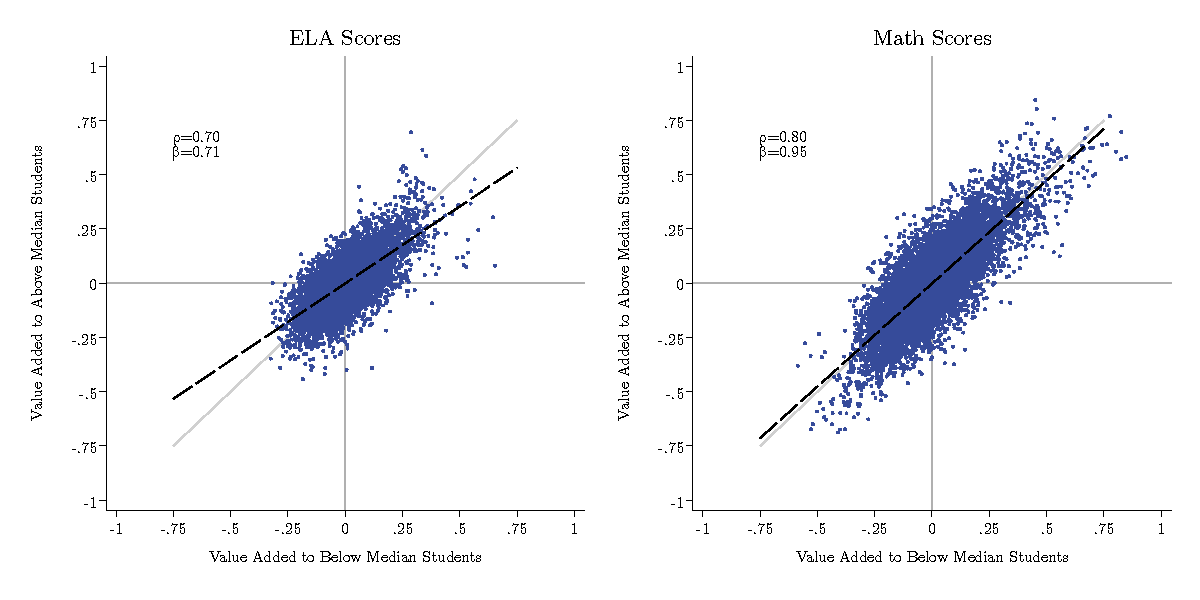
\includegraphics[width=.9\textwidth]{Working_Paper/test_figures/02a_VA.pdf}
    \caption{Value Added Varies Significantly within and across Teachers}
    \label{fig:va_est}
    \floatfoot{Note: This figure shows our heterogeneous estimates of teacher value added on both English Language Arts (ELA) and Math test scores. Each dot represents one teacher-year estimate of value added on high- and low-scoring students. The correlation coefficients is for the entire population stacked by year. The dashed line shows the line of best fit with the slope reported. For reference a line with slope one is plotted in the background.}
\end{figure}

Visual inspection of Figure \ref{fig:va_est} illustrates the differences within \textit{and} across teachers, suggesting we should reject the standard ``constant effects'' model of value in favor of one with appreciable comparative advantage. Differences across teachers, or absolute advantage, can be seen by comparing teachers along the gray 45-degree line. Teachers above and to the right generate larger testing gains compared to teachers below and to the left. Comparative advantage can also be seen visually. Teachers with dots above the gray 45-degree line have a comparative advantage in teaching high-scoring students, and teachers with dots below that line have a comparative advantage in teaching lower-scoring students. The size of the average comparative advantage is large: 53\% the size of the cross-teacher standard deviation in standard teacher value added for ELA and 48\% for math.  %Under the null of constant effects, we would expect all points to fall on the 45-degree line (up to sampling error), instead we see significant dispersion. Furthermore, the constant effects model implies both a slope coefficient and correlation coefficient of one---something that is not true in either exercise. 


The differences within and between teachers are what will generate gains for the reallocation exercises. We estimate that teacher value added to higher- and lower-scoring students is correlated at 0.7 for ELA and 0.8 for Math. The fact that this correlation is less than one allows for gains from allocating teachers by comparative advantage. Even though the correlations are high, there will still be significant margins for gains. For comparison, our cross-group correlations are lower than those by socioeconomic status \citep [0.9 for math in][]{bates2022teacher} but larger than those by race \citep[0.7 for math and 0.4 for ELA in][]{Delgado2020}. Furthermore, our theoretical framework suggests there is value in combining information from multiple outcomes. In that light, it is also worth noting that the cross-subject correlations are lower. For example Figure \ref{fig:A_va_est} shows that the cross-subject, cross-group correlations are both around 0.6, suggesting even larger gains from cross-subject comparative advantage

It is also interesting to note that Figure \ref{fig:va_est} reveals that value added to math is much more dispersed than value added to ELA. This is consistent with evidence from similar value added papers \citep[e.g.,][]{chetty2014measuring1} as well as with other research on the mathematical preparedness of elementary school teachers \citep{?,?,?}. Our results further show that teachers' value added is more highly correlated across achievement groups for Math than for ELA. This is also consistent with absolute advantage being more important and variable with Math teaching than with ELA teaching.



\subsubsection{Validation and Robustness}
Although these results suggest striking patterns of comparative advantage, our reallocation exercises and welfare estimates would be meaningless if these estimates reflected idiosyncratic noise rather than persistent heterogeneity within and across teachers. Although the use of shrinkage assuages these concerns, we also perform three additional exercises demonstrating the stability and credibility of our heterogeneous estimates. Each result reinforces our confidence that the value added scores are fitting systematic patterns in causal differences and not just idiosyncratic noise.

First, although a long literature on both traditional and heterogeneous value added estimates has repeatedly documented their forecast unbiasedness \citep[e.g.,][]{chetty2014measuring1,Delgado2020,bates2022teacher} we replicated these results in our own data. Appendix Figure \ref{fig:robust1} shows that heterogeneous value added scores are good out-of-sample predictors of student test-score growth. Second,  Appendix Figure \ref{fig:robust2} reports patterns of persistence over time. For example, over 40\% of teachers have a comparative advantage for teaching one group of students in \textit{all} years, and the year-to-year correlation is between 0.78-0.90 for all estimates.%and Appendix Table \ref{} reports the full auto(co)variance structure from behind our estimates.
 Finally, Appendix Figure \ref{fig:robust3} leverages the longitudinal nature of our data to show that heterogeneous value-added estimates carry the same information about long term outcomes as traditional value added estimates \citep{chetty2014measuring2}. These results show striking similarities between the effects of our estimates and traditional value added. Furthermore, estimates for each student group are no less precise suggesting that the variance is loading on the dimension of heterogeneity we specified.

\subsection{The Status-Quo Allocation of Teachers and Students} \label{squo}

This section shows how teachers are allocated to classes in the status quo, whether this allocation seems efficient or equitable, and presents descriptive evidence that there may be gains from reallocation.

Figure \ref{fig:squo1} shows that there is some sorting along absolute advantage. Higher value added teachers (using standard value added) are moderately sorted into classes with higher average test scores at baseline. This suggests the current allocation inequitable, but the effects are small (going from 1st to 99th percentile of share below median only predicts a reduction about 0.2 standard deviation reduction in value added which translates to just under a 0.03$\sigma$ student standard deviation difference in test score gains between the lowest and highest scoring classes.) Appendix Figure \ref{fig:squo2} shows analogous results by class size revealing that better teachers teach in slightly larger classes. This suggests some allocative efficiency from sorting better teachers in bigger classes, but again the differences are small. Interestingly, this effect may be tied to the inequities shown above since larger classes tend to be in more affluent schools with higher average test scores. These schools may tend to be more desirable for teachers in other dimensions.


The sorting on comparative advantage is less clear. In math, teachers who are comparatively better at teaching low-scoring students are sorting into classes with larger shares of low-scoring students, while the opposite is true in ELA. 


\begin{figure}[htpb]
\centering
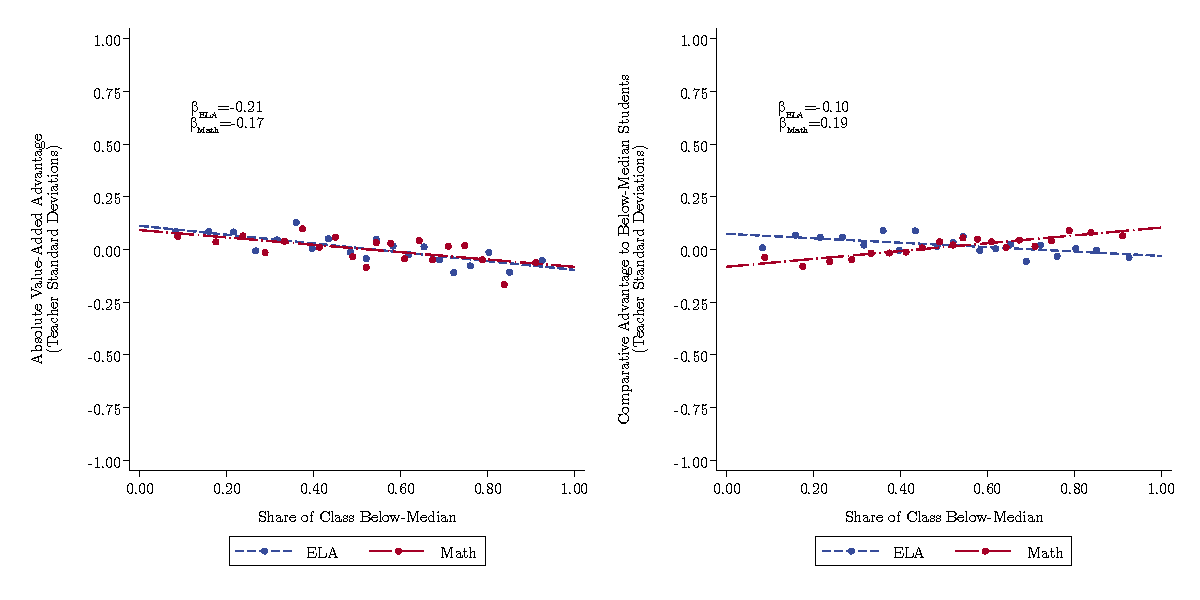
\includegraphics[width=.9\textwidth]{Working_Paper/test_figures/02_pct_low.pdf}
    \caption{Teacher Value Added Only Varies Somewhat with Class Composition}
    \label{fig:squo1}
    \floatfoot{Note: This figure shows how our heterogeneous estimates of teacher value added on both English Language Arts (ELA) and Math test scores relate to class composition. The panel on the left shows teacher absolute advantage (average of value added on above- and below-median students) and the panel on the right shows the comparative advantage (difference of value added on below-median students minus value added on above-median students). Both panel plot the ventiles of value added (measured in teacher standard deviations in absolute advantage) over the share of students who have below-median scores.}
\end{figure}



For standard value added or our heterogeneous value added approaches to lead to prescriptions for teacher reallocations that would improve welfare, several assumptions must play out in real-world data. For example, standard value-added models require class sizes to vary so that the ``best" teachers get the largest classes. Similarly, the heterogeneous value-added approach promises bigger gains from teacher reallocations only if classes vary in student mix. Table \ref{table:stddev1} shows that of these assumptions reflect the reality in the district we study. The first row shows the overall standard deviation in class size and the share of above-median students in math and ELA, after controlling for variations by grade times year. The second row removes across school variations, and thus shows the remaining and relevant variation should the policymaker only want to reallocate teachers within a school, by grade and year, rather than across schools. The table shows that ample variation in class size and the achievement composition of classes remains after controlling for school/grade/year means. 


\begin{table}[]


\begin{tabular}{ m{3.5cm}  m{3.5cm} m{3.5cm} m{3.5cm} }
After Control for: & Std. Deviation Class Size & Std. Deviation Share of Class Above Median, ELA Scores & Std. Deviation Share of Class Above Median, Math Scores   \\
Grade*Year         & 3.68                      & 0.50                                                  & 0.50                                                     \\
School*Grade*Year  & 1.71                      & 0.46                                                  & 0.46                                                     \\
                   &                           &                                                        &                                                          
\end{tabular}
\label{table:stddev1}
\caption{The Standard Deviation of Class Size and the Share of Students in the Class Who Are High-Scoring in ELA and Math}
\end{table}

Another notable finding from this table is that much of the variation in class size and in the composition of classes remains after controlling for grade by school by year fixed effects. The implication is that although reallocating teachers across schools necessarily allows for bigger test-score gains, much of the potential gains may be achievable by reallocating teachers within their current school and grade. (This matters in the district we study where teachers with the most seniority have priority when new slots open up. Put differently, this is a district in which teachers initiate inter-school moves, not administrators.)

% add table when get to final decision on how to correct bins.
Next we turn to the actual allocation of teachers to classes, with a view to assessing whether district administrators, in the years we studied, had any tendency to assign teachers strategically based on their absolute and comparative advantages, both within and between schools. To this end we 




\section{Efficiently Allocating Teachers to Classes}
\label{efficiently_allocating}
Although our general theoretical framework could be applied in many settings, with estimates of the heterogeneous teacher effects we now use our theory to consider the public service provision problem of allocating teachers to classes. This section defines the allocation problem, presents the gains possible under the optimal allocations, and compares the gains obtained from using our estimates relative to using traditional value added measures.

We parameterize the social objective $\accentset{\sim}{\mathcal{W}}$ using high and low scoring students to compare different allocations and find the relevant optima. Let $\mathcal{J}: (i,t)\to j$ be an allocation function, telling us which teachers teach each student in each year. We define the following optimization problem for weighted test score gains in a given subject ($s$ subject subscripts suppressed):
\begin{equation}\label{opt}
\max_{\mathcal{J}\in\mathscr{J}} \accentset{\sim}{\mathcal{W}}(\mathcal{J};\omega) = \max_{\mathcal{J}\in\mathscr{J}} \frac{1}{N_{i,t}}\sum_{(i,t)} \omega_{L} \,L_{i,t} \,\hat{\tau}^{\mathcal{J}(i,t)}_{L}  +(1-\omega_{L}) \, (1-L_{i,t}) \, \hat{\tau}^{\mathcal{J}(i,t)}_{H}
\end{equation}\noindent where $\omega_{L}\in[0.0,1.0]$ represents the weight on lower-scoring students in the social objective, $L_{i,t}$ is an indicator for whether student $i$ is lower-scoring, and $\hat{\tau}^j_{H}$ and $\hat{\tau}^j_{L}$ are our estimates of heterogeneous value added. The set $\mathscr{J}$ is the social planner's choice set made up of feasible allocations. In our setting, we focus only on reallocating teachers to existing classes in the grade they actually taught without changing the composition of those classes in any way. We do this to avoid introducing peer-effect biases into our welfare estimates.  The single-$\omega$ parameterization of welfare imposes linear indifference curves that trade off performance for lower- and higher-scoring students where the weight on each group reflects the degree to which the social planner wishes to target gains to on group of students relative to the other. It also assumes that the social planner only values gains to students in the given subject---something we will relax in Section 5.


%\footnote{Formally, each year $t$ all students $i$ and $i$'  must have the same teacher in all allocations or none: $\mathcal{J}(i,t)=\mathcal{J}(i',t)\iff \mathcal{J}'(i,t)=\mathcal{J}'(i',t)$, }

This allocation problem captures three distinct trade-offs that have been mentioned in the value added literature but never fully addressed. First, the optimal allocation must account for the \textit{comparative advantage} of teachers because of differences in \textit{class composition} \citep[as pointed out in][]{Delgado2020}. Second, the optimal allocation must also account for the \textit{absolute advantage} of teachers because of differences in \textit{class size}. This crucial detail has been accounted for at the school level \citep[see][]{bates2022teacher}, but class size and class composition vary both across \textit{and} within schools. Because of these differences, we are interested in both within-school and district-wide reallocation exercises. Finally, the optimal allocation must account for possible heterogeneity in the social value of gains to different types of students. 


We solve this allocation problem for two sets of possible reallocations: within-school and district-wide. For both, we restrict $\mathscr{J}$ so that every year the students in each class and the grade assignments of each teacher do not change. We leave class composition fixed so that changes in within-class peer effects do not contaminate the outcomes in predicted counterfactual allocations. For the within-school reallocation we further require that teachers do not change schools.  Whereas this within-school problem can be solved easily by iterating over school-grade(-year) cells, the district-wide reallocation problem has over $3\cross 10^{1830}$ allocations to search over. Because the optimal policy depends on both absolute and comparative advantage when both class sizes and class compositions vary, this problem cannot be solved by simply assigning teachers to classes with large shares of students they have a comparative advantage in teaching or simply assigning the best teachers to the largest classes. In Appendix \ref{optimization} we show that the social planner problem in equation \ref{opt} can be re-characterized as a mixed-integer linear programming problem and solved with [algorithm] \citep{?}



\subsection{Allocations Using Comparative Advantage Increase Test Scores}

We create a production-possibility frontier for the gains to each group from the within-school and district-wide reallocations. To do this, we solve the optimization problem in Equation \ref{opt} for 101 different values of the social weights $\omega_L$ ranging from 0.0 to 1.0. We then recover the average value added received by lower- and higher-scoring students and calculate the gain beyond the status quo. By comparing the optimal gains attained under different weights, this analysis characterizes how reallocation gains to lower-scoring students trade off with those to higher-scoring students, creating the production-possibility frontiers.

We depict these production-possibility frontiers in Figure \ref{fig:reallocation}. We plot the PPF for change in  ELA scores on the left and Math scores on the right. Each point presents the average one-year change in lower-scoring students' test scores in the optimal allocations (on the $y$-axis) over average change for higher-scoring students (on the $x$-axis), all relative to the status quo (noted with the square marker). Allocations that would reduce a group's scores relative to the status quo are denoted with negative numbers. Allocations above and/or to the right of the status quo are preferred by the social planner. The lighter (blue) PPF denotes the within-school reallocations and the darker (red) PPF the district-wide reallocations. Unsurprisingly, the district-wide reallocations produces gains that are further out in both dimensions.


\begin{figure}[htpb]
\centering
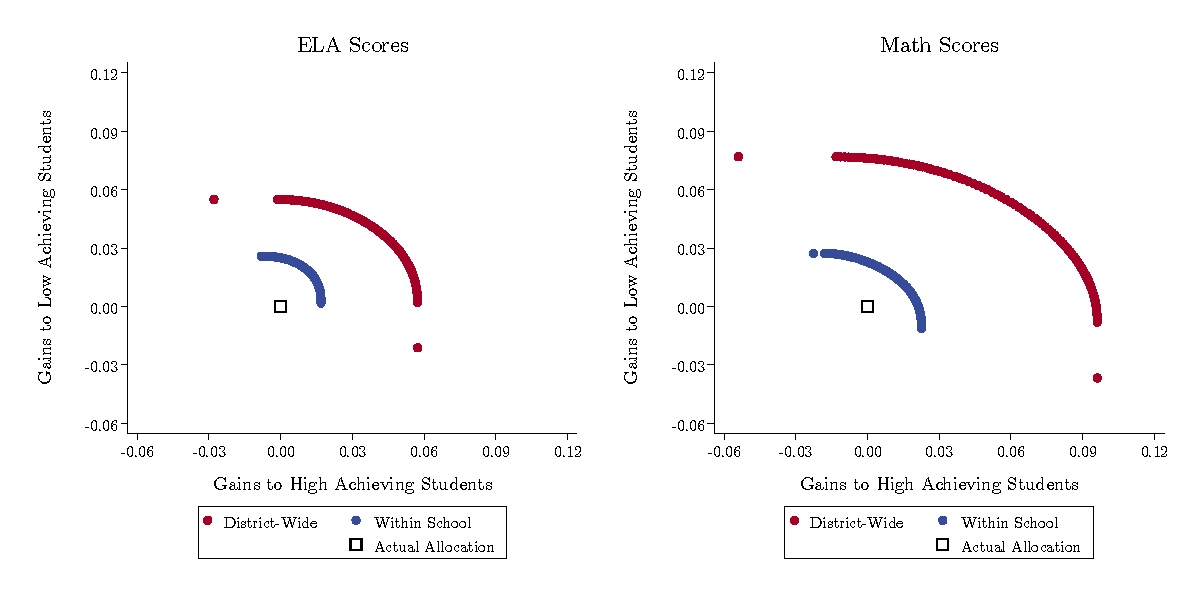
\includegraphics[width=.9\textwidth]{Working_Paper/test_figures/03_reallocation.pdf}
    \caption{Optimal Allocations Can Create Large Gains to High- and Low-scoring Students}
    \label{fig:reallocation}
    \floatfoot{Note: This figure shows the test score gains from optimal allocations relative to the status quo. Two production possibility frontiers are presented, one for reallocating teachers within school-grade cells and one reallocating teachers across schools (still within grade). Each PPF is constructed by finding the optimal allocation given relative weights on low- and high-scoring students [0.0,1.0] using the procedure described in Appendix \ref{optimization}. Gains are reported as average changes in scores measured in student standard deviations per school year that the reallocation is performed.}
\end{figure}

Figure \ref{fig:reallocation} reveals three striking patterns. First, there are large gains possible from both reallocations. For example, in the district-wide reallocation a social planner seeking to raise average scores (i.e., a utilitarian planner with $\omega_L=\omega_H=0.5$) could increase both lower- and higher-scoring students' scores by 0.04 student standard deviations. Gains from math are even larger: 0.04 for lower-scoring students and 0.07 for higher. Similarly, the simpler within-school reallocation could raise ELA and Math scores for both groups by more than 0.01 standard deviations. Recalling that these represent one-year gains, a policy that optimally allocated teachers could increase average math scores by $0.12\sigma$ in ELA and $0.17\sigma$ in math.\footnote{Where the annual means and standard deviations scores are normalized by those in the entire state of California.} These are large gains---almost identical to the gains that wold result from improving the value-added of \textit{every teacher} in the district by one teacher standard deviation (but retaining status quo assignments), and triple the gains from proposed teacher screening programs that ``deselect'' (i.e., fire) teachers with the lowest 5\% standard value added \citep[as considered in][]{hanushek2009teacher,hanushek2011economic,chetty2014measuring2}.

The second pattern visible in Figure \ref{fig:reallocation} is that the shape of these production possibility frontiers demonstrates the trade-offs between high and low scoring students in the reallocation exercises. For example, a policymaker who wanted to maximize the ELA (Math) scores of low-scoring students could generate  0.06$\sigma$ (0.08$\sigma$) in gains, but at the cost of 0.03$\sigma$ (0.05$\sigma$) to high-scoring students---although almost identical gains could be achieved without harming high-scoring students on average weighting them slightly more than zero. On the other hand a policymaker who wanted to maximize the ELA (Math) scores of high-scoring students could generate  0.06$\sigma$ (0.10$\sigma$) in gains, but at the cost of 0.02$\sigma$ (0.04$\sigma$) to low-scoring students---again with the possibility of similar gains without harming low-scoring students on average. The curvature of the PPFs at each point also reflects the gains that are possible without harming the other group. Furthermore, because  the choice of allocation matters based on the reallocation technology, picking an allocation that maximizes average scores isn't necessarily a  neutral choice. For example, in math it benefits higher-scoring students more. 


Finally, the distance between the white square marker for the status quo and the different frontiers can tell us a little about the district choices. While we cannot reverse engineer the social preferences that generate this allocation in our two dimensional space, the allocation could be on the frontier for some higher-dimensional preference. For example, a policymaker may value non-tested outcomes, respond to teachers' preferences for classes and schools, or care about some more nuanced subset of students (like the bottom or top achievement decile). While this could be part of the story, we expect there are institutional frictions and fixed costs of actually estimating heterogeneous value added that have prevented score-maximizing policies from being implemented. Regardless of the motivation for the status quo allocation, Figure \ref{fig:reallocation} shows that the current policy comes at the expense of average above- and below-median gains.
 

Estimating these gains highlights three interesting implications for our understanding of teacher allocations. First, the gains to math scores are larger than the gains to ELA scores. This is because the variance in teacher value added on math is larger as shown in Figure \ref{fig:va_est} and in prior work \citep[e.g.,][]{chetty2014measuring1}. This suggests that for one-subject reallocations like \citet{bates2022teacher}, it is indeed better to focus on math in order to raise average scores. Second, the allocations that optimize math scores and ELA scores are distinct. This is because the teachers that are the best at teaching each group of students math are not always the best at teaching those students in ELA. As such, the gains highlighted in papers that do reallocations using one subject at a time like \citet{Delgado2020} and \citet{bates2022teacher} only give a lower bound to the gains from using information on both outcomes simultaneously. This will motivate our analyses in Section \ref{welfare} where we aggregate gains over multidimensional outcomes. Finally, note that the largest possible gains to each group are different. This asymmetry highlights the welfare implications of structural features of the education system such as the fact that high-scoring students tend to be in larger classes compared to lower-scoring students. This class-size dimension becomes particularly important when comparing these allocations to those made using only information about absolute advantage from traditional value added estimates.

Before proceeding, we want to note three caveats in considering these reallocations. First, note that because we do not change class composition, these gains could be significantly larger in a district that employs class-level tracking because of greater variance in class composition. Second, the district-wide reallocations might be infeasible. For example, in SDUSD the union contract gives teachers with seniority higher priority in hiring. Furthermore, teachers have strong preferences over locations \citep{boyd2005a} and schools \citep{bates2022teacher} that could impede some allocations from being incentive compatible. Finally, the new allocations must be interpreted in the light of partial equilibrium, barring families re-sorting to classes (via requests), schools (via school choice), or districts (via in- or out-mobility).

\subsection{What Value Does Considering Heterogeneity Add?}
\label{considering heterogeneity}

The previous subsection quantified large gains from teacher reallocations, but how much of these gains would be possible without knowing the heterogeneous effects? If all of these gains simply come from moving better teachers to larger classes, there is no need to estimate heterogeneous effects. To evaluate the importance of estimating heterogeneity, we compare the best allocations using heterogeneous estimates with those possible using only standard estimates of value added. This allows us to decompose the welfare gains from the best allocations into the absolute advantage, comparative advantage, and redistribution components.

To find the optimal allocations with the standard value added we use the same set of social objective functions and same solution concept, but we replace the estimates of each teacher's value added on both higher- and lower-scoring students with the standard estimates:
\begin{equation}\label{opt2}
\max_{\mathcal{J}\in\mathscr{J}} \accentset{\sim}{\mathcal{W}}_{VA}(\mathcal{J};\omega) = \max_{\mathcal{J}\in\mathscr{J}} \frac{1}{N_{i,t}}\sum_{(i,t)} \omega_{L} \,L_{i,t} \,\hat{\tau}^{\mathcal{J}(i,t)}_{VA}  +(1-\omega_{L}) \, (1-L_{i,t}) \, \hat{\tau}^{\mathcal{J}(i,t)}_{VA}
\end{equation}\noindent where $\hat{\tau}^j_{VA}$ is the standard value estimate described in section \ref{va_std} and where we again solve the problem for 101 different values of the social weights $\omega_L$ ranging from 0.0 to 1.0.  Intuitively, the gains from using absolute advantage as captured in the standard measures come from putting the higher value-added teachers in larger classes to maximize average scores---or using $\omega_L$-weighted class size when the social planner has heterogeneous preferences over groups' gains. The gains attained and reported at each point are calculated using our heterogeneous estimates to avoid compromising the external validity of our score predictions that would occur if using standard estimates to predict the effect of sending teachers to very different classes. %Appendix Figure \ref{} illustrates the degree to which this extrapolation error would have biased the welfare estimates.

\subsubsection{Estimating Heterogeneity Increases Average Test Scores}
As illustrated in in Figure \ref{fig:theory}, the first mechanism by which using heterogeneous value added could increase average scores beyond what is possible using standard value added is through comparative advantage. This subsection explores the extent to which information about comparative advantages can raise average scores in practice. We document large gains beyond what can be accomplished using the information about absolute advantage from standard value added measures.

To approach this question, we depict and compare the production-possibility frontiers for average achievement gains to each group using heterogeneous and standard value added in Figure \ref{fig:va_versus}. Here again each point presents the average change in lower-scoring students' test scores in the optimal allocations (on the $y$-axis) over average change for higher-scoring students (on the $x$-axis). relative to the status quo (noted with the square marker). Panel (a) presents the results from the district-wide reallocation, Panel (b) presents those from the within-school reallocation. These figures also mark the allocations that maximize test scores with an X for reference---which is obtained by placing the highest value added teachers in the largest classes.

Note that the empirical results in Figure \ref{fig:va_versus} are analogous to the theoretical depiction in Figure \ref{fig:theory}. For each panel the outer PPF presents the changes in test scores possible by using information about both absolute and comparative advantage based on the heterogeneous teacher effects whereas the interior PPF presents the changes in test scores possible by using only the information abut absolute advantage contained in standard value added  estimates. Again the current allocation is denoted with a square.

\begin{figure}[htpb]
\centering
\begin{subfigure}{\textwidth}
\centering
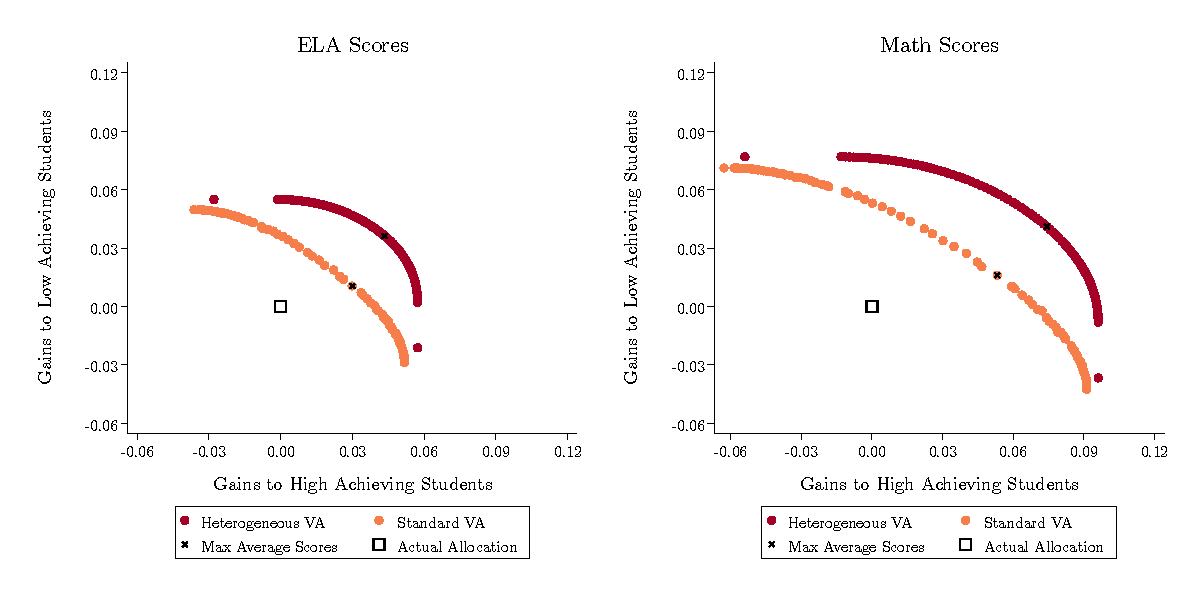
\includegraphics[width=.9\textwidth]{Working_Paper/test_figures/03a_versus_ac.pdf}
    \caption{District-Wide Reallocation}
 
\end{subfigure}

\begin{subfigure}{\textwidth}
\centering
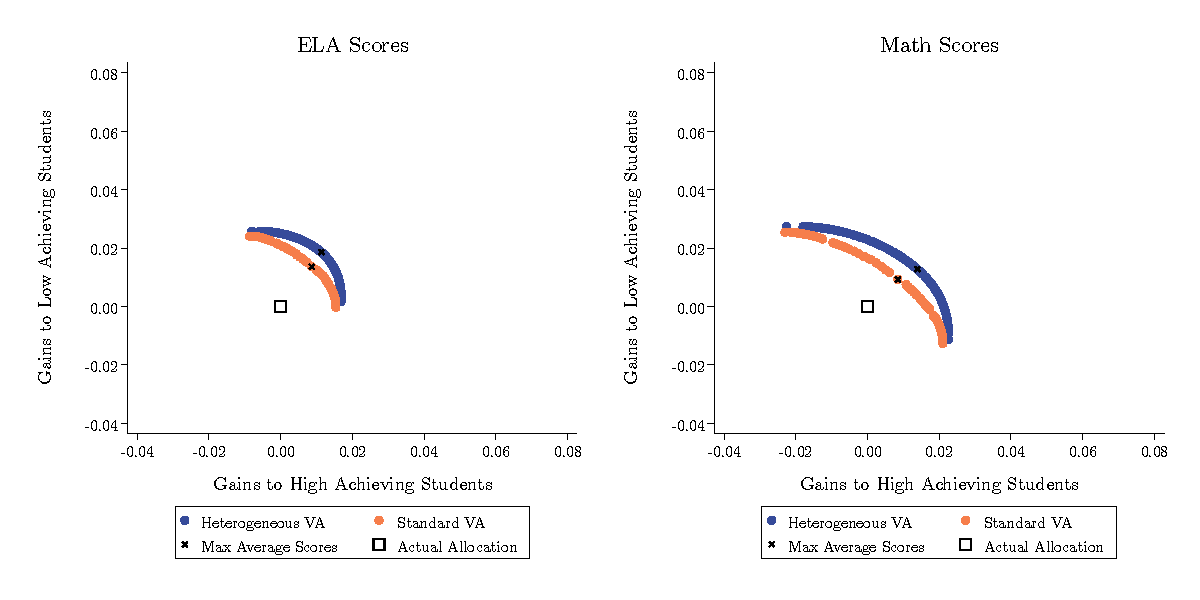
\includegraphics[width=.9\textwidth]{Working_Paper/test_figures/03b_versus_wi.pdf}
    \caption{Within-School Reallocation}
 
\end{subfigure}

    \caption{Using Heterogeneous Estimates Produces Larger Gains from Reallocation}
    \label{fig:va_versus}
    \floatfoot{Note: This figure shows the test score gains from optimal allocations relative to the status quo. In each panel two production possibility frontiers are presented, one for reallocating teachers based on our estimates of value added (absolute and comparative advantage) and one reallocating teachers only based on traditional value added (absolute advantage). Panel (a) displays the result for reallocating teachers across schools and panel (b) the results for reallocating teachers within schools (both always keep teacher in the same grade). Each PPF is constructed by finding the optimal allocation given relative weights on low- and high-scoring students [0.0,1.0] using the procedure described in the text (see details in Appendix 
    \ref{optimization}). Gains are reported as average changes in scores measured in student standard deviations per school year that the reallocation is performed.}
\end{figure}


Comparing the optimal allocations reveals that using information about comparative advantage can as much as double the achievement gains from reallocations. In the district-wide reallocation allocations using comparative advantage generate 97.3\% higher ELA scores and 66.4\% higher Math scores than allocations using only absolute advantage. These are large gains: an average gain of 0.020$\sigma$ in ELA or 0.023$\sigma$ in Math for \textit{every student} in the district would be an impressive policy victory, especially considering this policy could be implemented year-over-year for compounding gains. Gains to the within-school reallocations are smaller in absolute terms, but comparative advantage is still critical. Using heterogeneous effects boosts average ELA scores by 34.1\% and math scores by 50.3\% (both about 0.0045$\sigma$).

Interestingly, even for a social planner trying to maximize average scores the choice between standard and heterogeneous value added measures has striking distributional implications in the district-wide allocations. On one hand, the average-score gains from reallocations using only information about absolute advantage (from standard value added) are concentrated among high scoring students. For example the high-scoring students' gains of 0.03$\sigma$ in ELA  and 0.05$\sigma$ in Math are almost exactly three times larger than the corresponding gains to lower-scoring students.  On the other hand, the large gains from using comparative advantage in the  district-wide reallocations accrue disproportionately to lower scoring students. For example, the 0.02$\sigma$ ELA gain is split almost 0.03$\sigma$ to lower-scoring students and just over 0.01$\sigma$ to high-scoring students. Figure \ref{fig:va_versus} depicts these observations visibly: Whereas the expansion path from the status quo through the two PPFs is almost linear for the within-school reallocations in Panel (b), it is extremely non-linear for the district-wide reallocations Panel (a). These asymmetries motivate a direct focus on the equity implications of using heterogeneity.



\subsubsection{Accounting for Distributional Objectives Is Important}

The fact that using heterogeneous value added can increase average scores beyond what is possible using standard value added measures illustrates the importance of the ``comparative advantage'' channel highlighted in Figure \ref{fig:theory}, but this is not the only channel though which knowing heterogeneous value added can improve welfare. This subsection explores the additional distributional gains beyond those accomplished by raising average scores. These gains are dependent on the extent to which distributional goals deviate from the mean scores objective, but are large for more extreme distributional goals. 

%Perhaps surprisingly, we find that these gains are much smaller compared to the gains from matching.

%We make two comparisons to evaluate the interaction of heterogeneous value added and distributional objectives and report our findings in Figure \ref{fig:equity1}. First we compare the total welfare achieved under an optimal allocation (based on the welfare weights) relative to the test-score maximizing allocation. 

Using figure \ref{fig:va_versus} as a reference, we compare the total welfare achieved under an optimal allocation for a given set of welfare weights (the optimal point on the outer PPF for a given indifference curve) to the test-score maximizing allocation (the $x$ on the outer PPF). Specifically, we construct an ``Atkinson index'' type measure such that the social planner would be indifferent between the optimal allocation and an allocation where every student experienced a given test score gain. Figure \ref{fig:equity1a} shows the difference in this Atkinson index for each allocation on the comparative advantage frontier compared to the test-score maximizing allocation. As expected, the gains are zero for equal weights and grow as the social planner favors one group more or less. At the tail ends, where the policymaker favors one group almost exclusively, the gains for the within school reallocation are around .005$\sigma$ in ELA and .01$\sigma$ in Math. These are both larger than the .0045$\sigma$ gains from comparative advantage. Of course, the true weights for policymakers may not be near these tails, but this demonstrates significant potential for gains in the right setting.  

\begin{figure}[htpb]
\centering
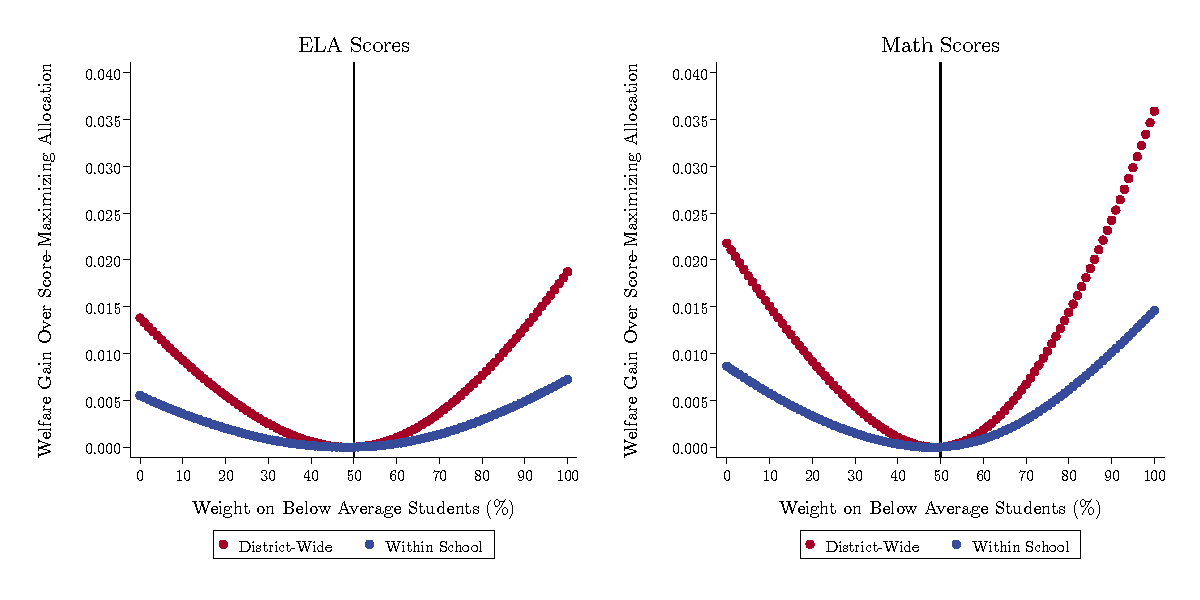
\includegraphics[width=.9\textwidth]{Working_Paper/test_figures/A3_redist.pdf}
    \caption{Welfare Gains from Considering Distributional Objectives}
    \label{fig:equity1a}
    \floatfoot{Note: This figure shows the differences in welfare attained under the score maximizing allocation and the optimal allocation using heterogeneous value added. The unit is an Atkinson Index indifference, i.e., how much would test scores have to increase for all students to generate equivalent welfare gains.  We report differences for both within-school and district-wide reallocations.}
\end{figure}

\subsubsection{The Interaction of Distributional Goals and Comparative Advantage}

The above sections show first that when the goal is to maximize average scores, considering comparative advantage using heterogeneous value added leads to significant gains. Second, when policymakers favor one group over another, considering their distributional goals also leads to significant welfare gains. Putting these together, we now address how different distributional objectives impact the gains from comparative advantage. 

Using figure \ref{fig:va_versus} as a reference, we are now comparing the welfare from the optimal points on the inner and outer PPF for a given distributional goal. Reporting the difference in the Atkinson index between the optimal allocation using standard and heterogeneous value added reveals the welfare gains from using heterogeneous value added estimates for a given distributional goal. Figure \ref{fig:equity1b} reports the results.  In Appendix Figure \ref{fig:equity3}, we present a simpler measure: the true (unweighted) difference in average scores for each pair of allocations. 


\begin{figure}[htpb]

\centering
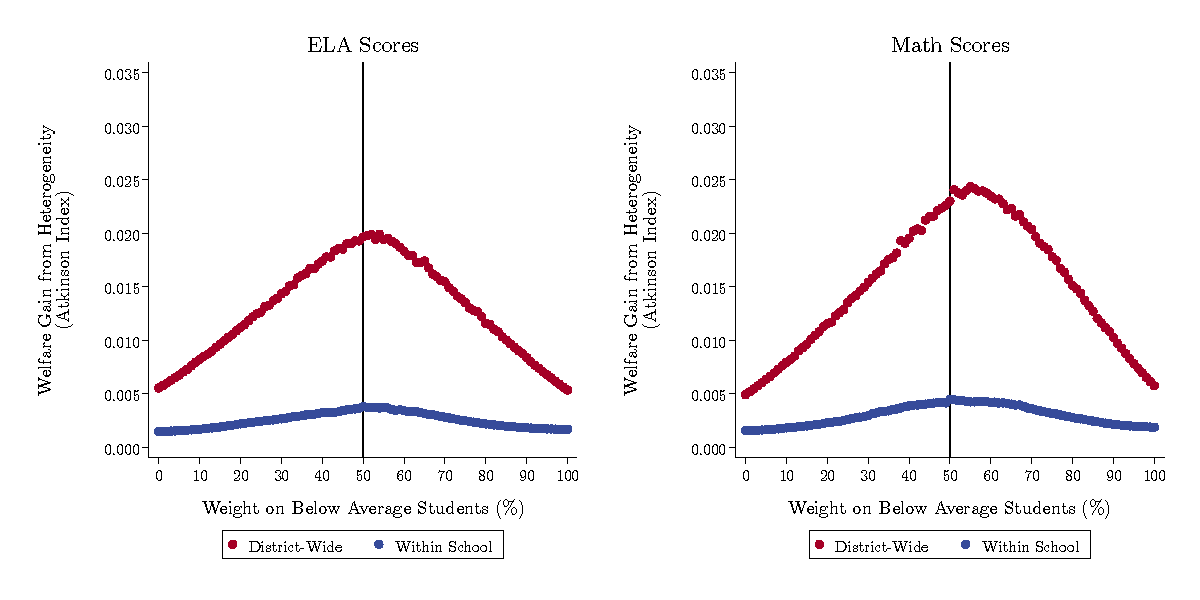
\includegraphics[width=.9\textwidth]{Working_Paper/test_figures/03f_reallocation.pdf}
    \caption{Welfare Gains from Comparative Advantage Along Distributional Objectives }
    \label{fig:equity1b}
    \floatfoot{Note: This figure compares the welfare attained at the optimal allocations based on our measures of value added with those attained at allocations based on standard value-added measures. The unit is an Atkinson Index indifference, i.e., how much would test scores have to increase for all students to generate equivalent welfare gains.  We report differences for both within-school and district-wide reallocations.}

    
\end{figure}

These analyses reveal that using heterogeneous value added matters most when the social planner has slightly egalitarian preferences. This is visible in Figure \ref{fig:equity1b} where for the district-wide reallocation the highest points on each upside-down U shape are slightly to the right of utilitarian preferences denoted with the gray line (at $\omega_L=\omega_H=0.5$). Although the maxima, where using heterogeneous value added is most useful, are at $\omega_L=$0.54 for ELA and 0.55 for math, the entire region between $\omega_L\in[0.30,0.70]$ show gains equivalent to over $0.015\sigma$ of gains to all students. 


The comparative advantage gains from estimating heterogeneous value added are only large if the social planner cares about both groups. For example, if the social planner only cares about lower- or higher-scoring students ($\omega_L\in\{0.0,1.0\}$), there are essentially no gains from comparative advantage using heterogeneous value added. This is because low- and high-scoring value added are positively correlated, so a policy that puts the highest absolute advantage teachers in the class with the most lower-scoring students will have a very similar effect on low-scoring students to a policy that puts the teachers with the highest below-median value added in the same classes. This is visible in how close the frontiers are in Figure \ref{fig:va_versus} and in the upside-down U-shape in the gains reported in Figure \ref{fig:equity1b}.


The key driver of these differences are the relative shapes of the PPFs and how they affect scores. As seen in Figure \ref{fig:va_versus}, the best attainable allocations using standard value added create a much flatter frontier than those using information about heterogeneity. As a result the ``price'' of an additional score increase to one group is much more expensive if the social planner relies only on information from standard value added measures. This has direct implications for average test scores, as seen in Appendix Figure \ref{fig:equity3}. Here we depict the change in average scores generated from moving from the optimal allocation attained using standard value added to the optimal allocation attained using our heterogeneous estimates. Rather than being U-shaped like the welfare gains, these suggest an M-shape where the score gains are biggest when on these flat regions of the interior PPF, but away from the center where average scores (and thus class sizes) are all that matter.


%In summary it seems like there are large welfare gains from using heterogeneous estimates, but that these occur mainly through the comparative advantage channel. 

In summery, comparative advantage and distributional goals are both potentially important to consider, but how they interact means one effect may play a much bigger role for a given policymaker. Redistribution is important when the social planner has very strong preferences for gains to one group relative to another; however, the standard measures of value added are able to capture most of these gains because value added heterogeneity is positively correlated within teachers.There is little scope for welfare gains from comparative advantage. Conversely, when a policymaker values gains to each group roughly equally, there is little scope for distributional gains to matter, but significant scope for welfare gains from comparative advantage. Since policy suggests some social objectives may be more nuanced we also turn our attention to the implications of our reallocations for achievement gaps and the creation of winners and losers.

\subsection{Other Equity Implications from Reallocations}

Having described the optimal reallocations and decomposed the welfare gains from them, our final task is to explore other equity implications that the proposed reallocations would have. Specifically we study how our reallocations affect achievement gaps and racial achievement gaps, and we describe how certain allocations that generate average gains still create significant heterogeneity for winners and losers masked by that average.

\subsubsection{Shrinking Achievement Gaps}

Many education policies---including those that motivated our welfare theory---propose interventions that will lower the achievement gaps between lower- and higher-scoring students. To consider this we plot out the change in two policy-relevant achievement gaps in Figure \ref{fig:equity2}. First, in Panel (a) we show how the optimal within-school and district-wide reallocations for each $\omega_L$ would change the achievement gap between students who performed above and below median in the previous year. We also report similar changes in the racial achievement gap in Panel (b). We define this gap as the difference in average scores between Black and Hispanic students versus White and Asian students. %\citep[following][]{}. 
Interestingly, we show that our completely race-blind policies can reduce average racial test score gaps just as much as the race focused reallocations in \citet{Delgado2020}.


\begin{figure}[htpb]
\centering
\begin{subfigure}{\textwidth}
\centering
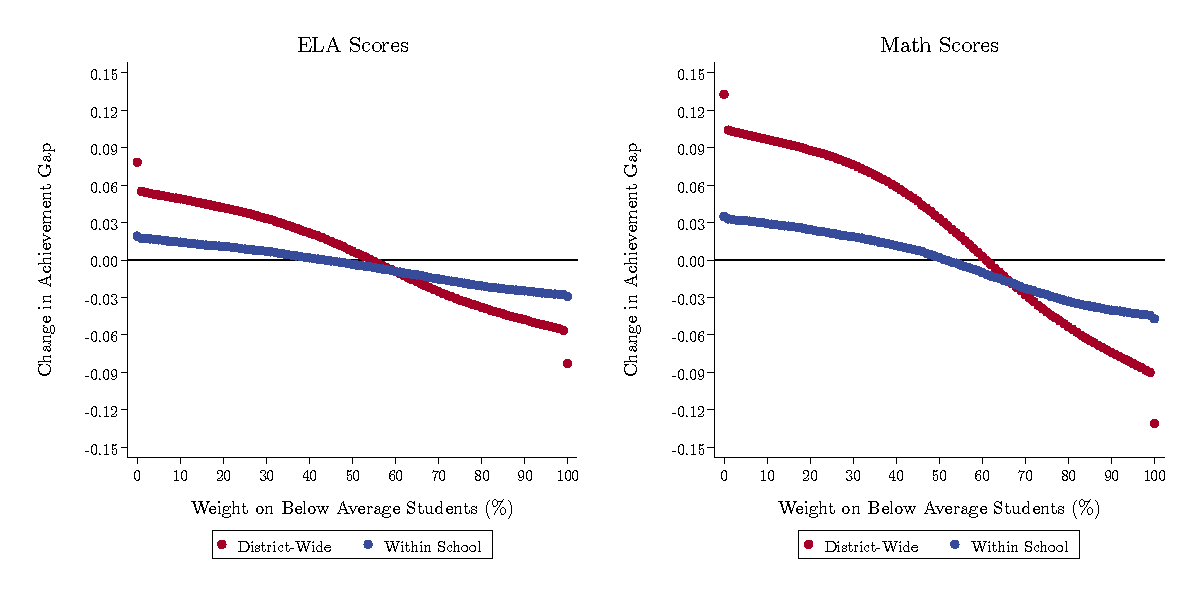
\includegraphics[width=.9\textwidth]{Working_Paper/test_figures/04a_gaps.pdf}
    \caption{Achievement Gaps}
 
\end{subfigure}

\begin{subfigure}{\textwidth}
\centering
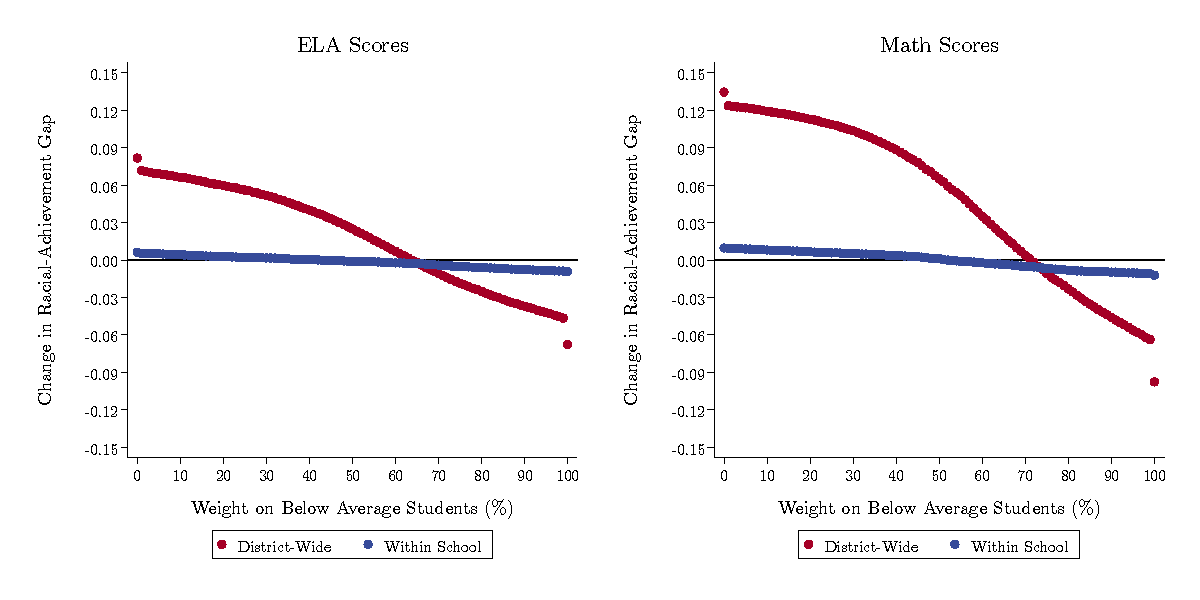
\includegraphics[width=.9\textwidth]{Working_Paper/test_figures/04b_gaps.pdf}
    \caption{Racial-Achievement Gap}
 
\end{subfigure}

    \caption{Reallocations Can Shrink Persistent Gaps in Student Performance}
    \label{fig:equity2}
    \floatfoot{Note: This figure shows how optimal reallocations would change achievement gaps between students. Each panel plots the change in the gaps of interest over the relative weights on high- and low-scoring students. Panel (a) displays the change in the average difference in test scores between students who scored below versus above the median in the previous year (relative to about 1.2$\sigma$), and Panel (b) displays the change in the average difference in test scores between Black and Hispanic students versus white and Asian students (relative to about 0.7$\sigma$). Both gaps are measured in student standard deviations.}
\end{figure}


The main takeaway from these analyses is that a social planner who cares about gaps can partially control the size of the gaps by making allocations that are on the efficiency frontier based on comparative advantage. For example, the baseline gap between students who scored above and below the median last year is 1.27$\sigma$ in ELA and 1.19$\sigma$ in Math. A social planner focused on raising lower-scoring students scores without, on average, hurting higher-scoring students could shrink those gaps by 4.4 and 7.6\% \textit{every year}. The gap between Black and Hispanic students versus white and Asian students are smaller: at 0.72$\sigma$ in ELA and 0.63$\sigma$ in Math, and these gains could be reduced by 6.5\% and 9.7\% per year. These changes are strikingly similar to those in \citet{Delgado2020} where allocations are made to explicitly shrink racial gaps in math scores subject to not lowering average scores.\citet{Delgado2020} finds a 0.068$\sigma$ reduction in the racial gap with no change in average scores, but using a race blind policy our district-wide reallocations would shrink the gap by 0.064 and \textit{raise} average test scores by 0.032$\sigma$. \footnote{Note that in our context larger reductions in gains are obviously possible if the social planner is willing to choose allocations that actually reduce the average scores of certain groups while staying on the frontier. While it is likely that there are interior allocations in which gaps could be further reduced, we restrict our focus to allocations that are on the frontier of gains to high- and lower-scoring students.} 

There are three additional points we want to highlight from this figure with implications for which gaps are effected. First,  whereas both the within-school and district-wide reallocations could change the achievement gap, only the district-wide reallocations could meaningfully affect the racial achievement gap. This makes sense because there is more variance in racial composition across schools than within. 

Second, it is interesting to note that the welfare weights that hold gaps constant vary a lot across allocations. For the within-school reallocations attaining similar gaps requires a weight on lower-scoring students between 40-43\% for ELA and 52-53\% for Math. On the other hand the district-wide reallocations require much larger weights on lower-scoring students. For example, it takes 55\% and 61\% to shrink the achievement gaps in ELA and math, and even more to shrink the racial gaps: 64\% and 72\%. For context, this means that to control the racial-achievement gap in math, the a social planner would have to forego 0.007$\sigma$ in average gains.


Finally, although utilitarian test-score maximizing reallocations ($\omega_L=\omega_H=0.5$) within school tend to not affect either gap significantly,\footnote{In fact, if anything they would slightly shrink the achievement gap.} district-wide reallocations to maximize test scores will actually expand both the achievement and racial achievement gaps. Intuitively this is because of cross-school co-variation in achievement (or race) and class size as discussed above.


\subsubsection{Reallocation winners and losers}

As noted above, because there are so many students, no reallocation---even one creating large average gains---is a Pareto gain in the sense that it helps, or leaves unaffected, all students. Despite the net gains from matching teachers to their comparative advantages and putting stronger teachers in larger classes, reallocations will assign some students to less effective teachers or to teachers who are a worse match for them (despite the teacher being a better match for their class). 

Before communicating these results, we want to highlight the fact that \textit{any} allocation of teachers to students will assign some students better teachers than others. In that sense the ``harms'' presented here should be benchmarked by the fact that in the status quo roughly one third of students are assigned to a teacher with below-median value each year (among teachers teaching the relevant grade in the students school), and for these students, the average ``loss'' (relative to the expectation) is about 0.10 student standard deviations in their scores on tests of each subject. Furthermore, students who attend schools with the lowest quartile of teacher value added tend to experience gains XXX smaller than students who attend schools with the top quartile of value added.

With that context in mind, Appendix Figure \ref{fig:harms} shows that just as some students experience lower test score growth because of the year-to-year allocations of teachers in the status quo, some also receive lower value added teachers in our reallocations. For example, the optimal within-school reallocations assigns between 35-38\% of students to lower value-added teachers, with 39-47\% for the district-wide reallocations. Unsurprisingly, more egalitarian allocations reduce the achievement gains of higher-scoring students relative to the status quo whereas more elitist allocations reduce the gains to more lower-scoring students. Appendix Figure \ref{fig:harms} also reports the average achievement loss among students who are harmed. In the optimal district-wide (within-school) allocations, students who receive lower value-added teachers than they would in the status who experience 0.104-0.120$\sigma$ (0.085-0.099$\sigma$) smaller ELA testing gains on average and 0.173-0.204$\sigma$ (0.140-0.165$\sigma$) smaller math gains on average, per year. While these figures sound large in terms of educational interventions, it's important to remember that they are relatively similar to the ``losses'' that are occurring in the status quo. Our reallocations change which students receive teachers with lower absolute advantage or poorly matched comparative advantage, but on average these changes are more than offset by even larger average gains to other observably similar students.


One implication of this depiction of winners and losers is that our reallocative policies have a strong redistributive component. For a social planner who only cares about higher- versus lower-scoring students this consideration is irrelevant, but in practice districts may want to preserve some horizontal equity.\footnote{At least relative to the status quo. In an obvious sense, the opportunity cost of the current allocation is that it harming (or at least not benefiting) many students that a different allocation could be making better off.} For example, because our reallocations tend to put teachers with higher absolute advantage in larger classes and because larger classes  tend to be in schools with more higher-scoring students, our optimal  reallocations will tend to benefit lower-scoring students in these schools slightly more than lower-scoring students in schools with lower average achievement. As discussed in Section \ref{theory_section}, this may be troubling if the policymaker has preferences over multiple dimensions of student characteristics. For example, this could be problematic if the policymaker is most concerned about low-scoring students in schools with lower achievement given the importance of school disadvantage in student learning and long-term outcomes \citep[e.g., see][]{}.


The fact that there are indeed winners and losers among students, in addition to the observation that teachers, administrators, and teachers' unions---by revealed preference---weakly prefer the status quo to any reallocation raises the question of welfare implications from these reallocation policies. Can schools reallocate teachers in ways that matter for welfare? How could they make such reallocations incentive compatible for families and teachers? What would be the cost of smoothing such incentive compatibility constraints? And would the reallocation still be worth doing? These are questions we consider in the following section.

\section{From Value Added to Welfare Added} \label{welfare}

% the above section can be seen as simply information about test scores. But, using our welfare theory, this work may provide an unbiased estimate of welfare.
We have provided a welfare theory, estimated the relevant parameters, and demonstrated the test score gains from reallocations along a single subject. Our empirical findings so far can be interpreted as statements about a popular outcome of interest, test scores. With some assumptions, however, our findings on test score gains can be interpreted as an unbiased, or less biased than the mean, welfare estimate using our welfare theory. 

%Having provided a welfare theory, estimated the relevant parameters, and demonstrated the gains from reallocations along a single subject, we now turn our attention to the welfare considerations of policies. Until now our reallocations have assumed that the social planner is maximizing a social objective based on test scores in one subject.  In this section, we expand the scope of our analyses to consider welfare improvements as measured in dollars to both students and teachers. This extends our insights from focusing only on one dimension of student achievement.

First, we need to make an assumption about family preferences and their behavior in light of our policy change. We assume that families---the main decision-makers for students--- value the average achievement of the school they enroll in. This means that students will not re-sort to new schools after we have rearranged teachers within a school. This is obviously restrictive as parents value many aspects of education, some idiosyncratic, like having a teacher an older sibling took classes from \citep[][]{}, and others more systematic, like the non-cognitive value added of teachers or schools \citep[][]{jackson2018test,pope2017multidimensional}. Nevertheless, the vast majority of families do not request specific teachers, and even when they do, not all requests are honored. %\citp{tannerspapers}. 
This assumption is analogous to the ``no spillovers'' condition assumed in Section \ref{theory_section}. Given extensive evidence that families do not respond to information about value added in school choice \citep{abdulkadirouglu2020parents} or housing markets \citep{imberman2016does}, we think this assumption is not too restrictive. Readers critical of this assumption should consider all welfare gains in partial equilibrium terms.

Second, we need to consider the bias terms from theorem \ref{thm_cond_bias}. First, consider the covariance term. It is important to remember that this term is dependent on the policymaker's welfare weights. As mentioned above, the covariance terms would be zero if our policymaker truly cared about only average low- and high-scoring students. If this is not the case, for a completely unbiased estimate, we need the conditional covariance of the true welfare weights (that consider all factor important to the policymaker) and student gains to be uncorrelated. we know that different allocations impact racial test score gaps and that gains from some reallocations accrue to low-achieving students primarily in high-achieving schools. While the estimates may not be unbiased in this case, satisfying equation \ref{eq:cond_ineq_cov2} would still ensure they are better than simple means. Conditioning on additional factors like race and school average scores could further assuage these concerns, but for tractability, we stick to conditioning on test scores. 

Next, we consider the estimation bias between our estimated conditional average treatment effect and the truth. While we know teacher impacts differ along different dimensions \citep{Delgado2020}, we believe conditioning on test scores captures much of the variation without over-fitting. While race also plays a role, finding common support for all teachers can be practically challenging. Gender may play a role in teacher impacts as well, however, gender composition does not change significantly between most classes, limiting the bias introduced by teacher heterogeneity. 

There are still two significant shortcomings that we address in the following section. First, these teacher's teach both ELA and Math, and so an optimal reallocation policy would consider the impact on both simultaneously. To combine both of these subjects into a single score function, we map achievement gains to lifetime earnings, which we do using the subject-specific estimates from \citet{chetty2014measuring1} of how value added affects lifetime earnings.


 %We make two main assumptions about family preferences and behavior to approach their contribution to welfare. First we assume that families---the main decision-makers for students---value two things: the present value of life time earnings from achievement and the average achievement at the school they enroll in. This is obviously restrictive as parents value many aspects of education, some idiosyncratic, like having a teacher an older sibling took classes from \citep[][]{}, and others more systematic, like the non-cognitive value added of teachers or schools \citep[][]{jackson2018test,pope2017multidimensional}. Nevertheless, the vast majority of families do not request specific teachers, and even when they do not all requests are honored. %\citp{tannerspapers}. 

% Similarly, assuming future earnings fully capture the impact of test score gains on well-being is a simplification.%, but we will show that our  achievement-optimal allocations leave teacher value added to social and behavioral outcomes unchanged on average within groups
%\footnote{Another way to interpret this assumption less restrictively is with a Koldor-Hicks style argument \citep{Hicks_1940,Kaldor_1939} that since total present value income is increased, lump sum transfers could be made to achieve a Pareto-gain.}. 
%The main empirical challenge is mapping achievement gains to lifetime earnings, which we do using the subject-specific estimates from \citet{chetty2014measuring1} of how value added affects lifetime earnings.

%
%The second assumption is that the teacher reallocations are taken as partial equilibrium, such that families to not try to re-sort to schools within the district and so that families do not leave or come to the district because of the policy. This assumption is analogous to the ``no spillovers'' condition assumed in Section \ref{theory_section}. Given extensive evidence that families do not respond to information about value added in school choice \citep{abdulkadirouglu2020parents} or housing markets \citep{imberman2016does}, we think this assumption is not too restrictive. Readers critical of this assumption should consider all welfare gains in partial equilibrium terms. 

The second shortcoming to address is the impact of reallocations on teachers. We need to consider the welfare component attributable to teachers' disutility from the reallocations. We treat teacher's preferences as an incentive compatibility constraint and assume they will need to be compensated enough to willingly switch classes. Using a revealed preference argument, if teachers willingly move, they will have been made better off. Assuming all teachers must be compensated for changing assignments will likely overstate the cost to teachers because at least some may prefer their new assignments,\footnote{For example, some teachers will be sent to schools they would like to teach at but cannot because of opening and union tenure requirement.} the main challenge is how to price this disutility. Some papers have attempted to price the disutility to teachers from various policies \citep[e.g.,][]{rothstein2015teacher,bates2022teacher}, but highly structured wages in teacher labor markets often make this difficult in practice. We will focus on the the marginal value of public funds \citep[MVPF,][]{Keyser_2020} for a hypothetical universal bonus program. %relying on estimates of teacher willingness to pay \citep{myabejohnstonpaper?} to evaluate incentive compatibility.


Note that by restricting our focus on families and teachers in this way, we implicitly assume that other considerations like union concerns or the administrative costs of performing the reallocations are negligible. While these considerations are likely important, we argue that welfare gains of a large enough magnitude could allow transfers or interventions to alleviate these concerns or pay these costs.


\subsection{Students: Earnings Implications of Reallocations}

We begin with the welfare implications for students under the assumptions outlined above. These results are most closely tied to our previous analyses focused on student gains. This subsection demonstrates our approach for finding the optimal achievement gains for students' lifetime earnings and performing allocations that maximize those income gains. 

\subsubsection{Choosing an Income-Optimal Score Function}
Because there are numerous allocations, all of which would generate different earnings outcomes, our first objective is choosing a welfare ``score'' function to maximize income. To do so we use the subject-specific estimates of the effects of value added in Math or ELA on student earnings from \citet{chetty2014measuring1}. They estimate that a one standard deviation increase in ELA scores in elementary school generates an additional \$1,524 in earnings in early adulthood and that the corresponding gains in Math are \$650. 

Because of the fundamental trade-off between the facts that our reallocations generate larger gains in math, but gains to ELA matter more for earnings, we take a principled approach to defining the income-optimal allocation. We consider the following set of utilitarian score functions that take into account value added in two subjects, $s$, ELA and Math.\footnote{We will soon relax the assumption about a utilitarian social planner.}
\begin{equation}
\accentset{\sim}{\mathcal{W}}(\mathcal{J};\omega) =  \frac{1}{N_{i,t}}\sum_{(i,t)} \sum_{s} \omega_s \left [ L_{i,s,t} \,\hat{\tau}^{\mathcal{J}(i,t)}_{L,s}  + (1-L_{i,s,t}) \, \hat{\tau}^{\mathcal{J}(i,t)}_{H,s} \right ]
\end{equation}
\noindent where $\omega_s$ represent the weight on each subject and $\sum_s \omega_s = 1$. And now $L_{i,s,t}$ indicates whether the student is low scoring in that particular subject.

Solving the optimization problem for a range of $\omega_{ELA}\in[0.0,1.0]$ generates a production possibility frontier similar to those in the reallocation exercises in Section \ref{efficiently_allocating}. Whereas the previous PPF plotted the trade-offs of possible gains between higher- and lower-scoring students, the PPF in Panel (a) of Figure \ref{fig:dollars} presents the trade-offs between gains to average Math and average ELA scores. For example, an allocation focused entirely on Math scores could raise average math scores by 0.058$\sigma$ (0.016$\sigma$ within schools).  Because Math and ELA value added are somewhat correlated, this allocation would also raise ELA scores by 0.019$\sigma$ (0.005$\sigma$ within schools). The focus on math scores only, however, forgoes large ELA gains. This could be particularly problematic as ELA gains are nearly 2.5 times more important for earnings.


We combine the information on possible gains with the estimates of the subject-specific income effects of those gains to calculate the weight each subject that maximizes income gains. The estimates from \citet{chetty2014measuring1} create relative ``prices'' of gains to scores in each subject measured in earnings. As such, the income-maximizing weight sets the marginal rate of substitution between ELA and math scores equal to the relative price. We illustrate this graphically in Panel (a) of Figure \ref{fig:dollars} using a dashed line with a slope of the relative price. This line is tangent to the within-school PPF at $\omega_{ELA}=0.71$ and to the district-wide PPF at $\omega_{ELA}=0.70$. %Appendix Figure \ref{} shows that for most non-utilitarian welfare weights that value gains to both groups of students, the optimal weight on ELA gains is in the range of 0.?? to 0.??. 
These values favor ELA gains, but do not focus exclusively on ELA value added because the value of marginal gains to ELA scores from increasing $\omega_{ELA}$ beyond 0.71 are smaller than the value of the larger gains to increasing math scores.


The combination of gains from both subjects significantly increases the income gains from students.
The facts that math value added scores have higher variance and result in larger achievement gains from reallocations might motivate a social planner to focus only on math scores in their objective function. In fact, this intuition plays out in the policy experiments considered in \citet{Delgado2020} and \citet{bates2022teacher} which both focus only on math. Surprisingly, our results overturn this intuition. We will discuss the details of how we obtain these numbers below, but we find that a district-wide allocation that focuses only on math scores increases average present-valued earnings by \$1030. The insight that we can incorporating information about both math and ELA optimally generates gains of \$1390 per student. This \$360 (34\%) gain is large and is costless once one allows the social planner to optimally weight value added to both test scores.

\begin{figure}[htpb]
\centering
\begin{subfigure}{\textwidth}
\centering
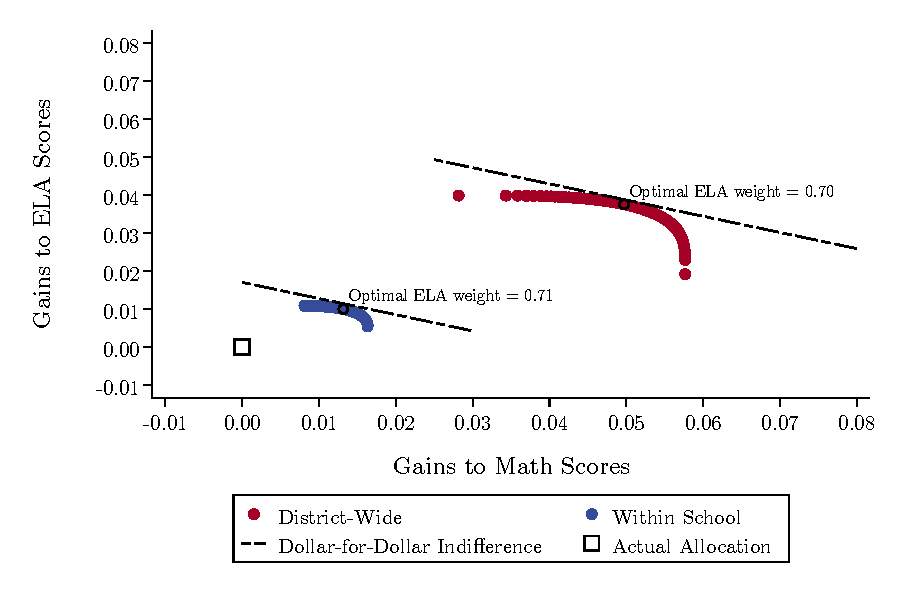
\includegraphics[width=.7\textwidth]{Working_Paper/test_figures/05c_dollars.pdf}
    \caption{Choosing the Wage-Maximizing Score Function}
\end{subfigure}

\begin{subfigure}{\textwidth}
\centering
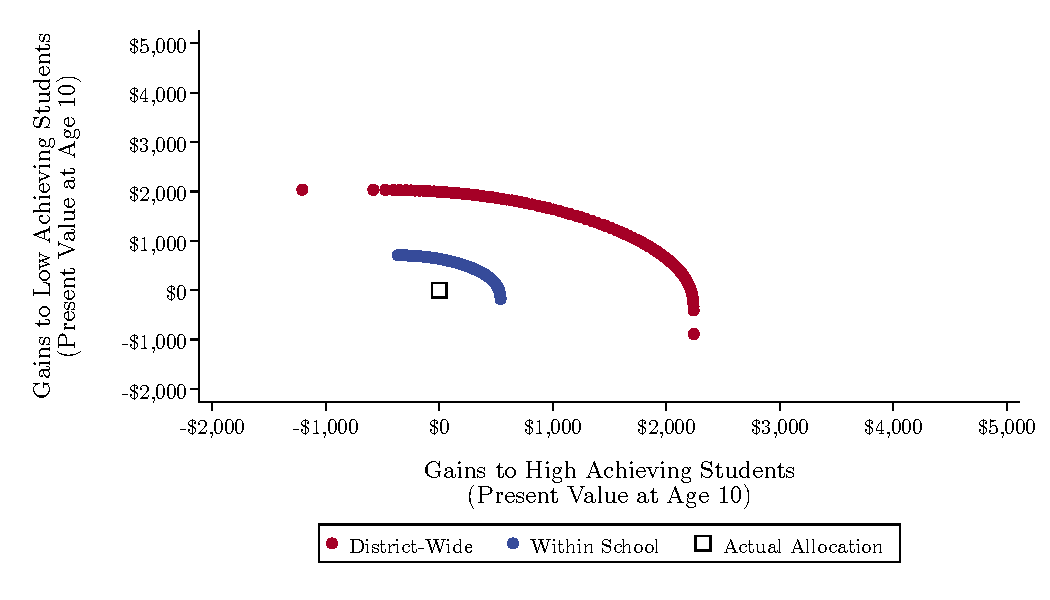
\includegraphics[width=.75\textwidth]{Working_Paper/test_figures/05d_dollars.pdf}
    \caption{Present Value Income Gains}
\end{subfigure}

    \caption{Reallocations Can Shrink Persistent Gaps in Student Performance}
    \label{fig:dollars}
    \floatfoot{Note: This figure shows how we combine math and ELA scores to estimate the frontier of possible earnings gains. Panel (a) displays the PPF of math versus ELA gains (assuming equal weights). The tangent lines are those implied by the subject-specific estimates of \citet{chetty2014measuring1}. Panel (b) shows the implied effect on lifetime earnings from reallocations with a score of S =0.75 ELA + 0.25 Math (present valued at age 10). }
    
\end{figure}

\subsubsection{Characterizing Possible Income Gains}

With information about the income-optimal score function in hand, we return to the question of 
optimal policy with hetereogeneous social preferences. Combining all of the pieces we define a new social welfare function to optimize
\begin{align*}
\accentset{\sim}{\mathcal{W}}(\mathcal{J};\omega) =  \frac{1}{N_{i,t}}\sum_{(i,t)} \omega_L &\left [\omega_{\text{ELA}} \, L_{i,\text{ELA},t} \,\hat{\tau}^{\mathcal{J}(i,t)}_{L,\text{ELA}}  + (1-\omega_{\text{ELA}}) L_{i,\text{Math},t} \,\hat{\tau}^{\mathcal{J}(i,t)}_{L,\text{Math}} \right ] \\
+(1-\omega_L) & \left [\omega_{\text{ELA}} \, (1-L_{i,\text{ELA},t}) \,\hat{\tau}^{\mathcal{J}(i,t)}_{H,\text{ELA}}  + (1-\omega_{\text{ELA}}) \, (1-L_{i,\text{Math},t}) \,\hat{\tau}^{\mathcal{J}(i,t)}_{H,\text{Math}} \right ]
\end{align*}
\noindent where now we explicitly sum test score gains over both subjects and both student types with their respective weights. Because this formulation exponentially increases the dimensionality of $\omega$, we use our evidence about income-optimal weights to choose $\omega_{\text{ELA}}=0.75$  and $\omega_{\text{Math}}=0.25$ in this section. To the extent to which the optimal $\omega^*_{\text{ELA}}$ varies over $\omega_L$, our results provide a lower bound on the true earnings gains.\footnote{Note that because not all students are low scoring in Math and ELA the achievement weight $\omega_L$ may not apply uniformly to each student. In practice this means that there are four implicit weights generated by this welfare function. One conceptually simple way to think of this function is treating each student's score as a different student and then weighting the welfare from gains to that ``student'' by both their achievement and which test it is.}

After calculating the efficient allocations for each $\omega$, we use the process in \citet{chetty2014measuring1} to map the test score improvements into the present value of lifetime earnings. We outline our approach as follows. First, we assume that individuals may choose to work between the ages 20 and 65. We also assume that the average income gains implied from test scores apply to all of these earning. Finally, we assume that families discount these earnings gains at a 3\% (i.e., with a 5 percent discount rate partially offset by 2 percent wage growth) back to age 10, the average age of students in our sample. Empirically this implies a multiplier of 15.5 on the baseline gains implied from test scores.

The results, depicted in Panel (b) of Figure \ref{fig:dollars} show that optimally reallocating teachers could create millions of dollars of gains per year. Based on our calculation, the income-maximizing district-wide allocation would generate over \$1140 in present valued earnings for low scoring students and over \$1630 for high-scoring students. Since there are 10,150 students of each type each year (on average), this implies the value of the reallocation across all students is  \$27.9 million. While smaller, the gains from the within school reallocations are not insignificant: over \$400 for lower-scoring students and over \$300 for high-scoring students, implying \$7.4 million across the district.

Policy makers concerned about inequality can also create large redistributive gains. For example in the district-wide reallocation, a social planner could increase the present value of lower-scoring students' earnings by \$1990 without hurting high scoring students on average. A similar comparison reveals gains of \$600 from within school reallocations. Compounded year-over year gains like these could be powerful tools at reducing not only achievement, but also earnings inequality among students coming out of the district. In Appendix Figure \ref{fig:ces}, we compare these results to those of a social planner with continuous CES preferences across students rather than discrete preferences across groups and show similar patterns.  

Taken together the gains from this policy are enormous. Even if the 27.9 million dollar gain is infeasible because of teacher or union preferences, the within-school reallocation is an essentially costless program generating nearly quarter of those gains. This compares very favorably to other elementary school interventions like .... \citep[][]{}, .... \citep[][]{}, and .... \citep[][]{} and underscores the power of using information about comparative advantage to improve policy. Furthermore, if there are ways to make the 27.9 million dollar gains attainable, a discussion of how to do so is of first-order importance. The following subsection provides that discussion.

\subsection{Teachers: Welfare Value of a Teacher Bonus Program}

We now turn to the welfare implications for teachers. Rather than trying to price teacher disutility, we focus on a teacher bonus thought experiment. One advantage of considering this experiment is that it allows us to separately consider welfare and incentive compatibility. Our estimates reflect the welfare attainable for each policy and would allow policymakers to choose the optimal one based on their understanding of the incentive constraints (e.g., teacher supply, wages, ammenities, senority, unions, etc.).

%(something that rigid wage and seniority schedules would complicate in the SDUSD context), .


Imagine a policy that paid all teachers a certain bonus for participating in a reallocation. Teachers would be paid this bonus whether or not their school or class assignment changed. If the bonus was sufficient to ensure incentive compatibility, then one way to characterize the welfare under the resulting allocation would be the marginal value of public funds \citep[MVPF,][]{Keyser_2020}. This characterizes a lower bound on an envelope of possible incentive programs that could be improved by targeting bonuses the teachers with the highest impacts from reallocation or by relaxing the requirement to participate in the reallocation (for example, for teachers with very strong preferences to their current assignment.

The MVPF is a ``bang-for-the-buck'' measure of the bonus program, calculated as the present value of the total program benefits divided by the net cost of implementing it. Specifically, for a bonus of size $b$ the MVPF of allocation $j$ is
\begin{equation}\label{mvpf_eq}
MVPF^j(b) = \frac{\sum_i (1-t)\Delta S^p_i)}{N_j b - t\Delta S^p_)}    
\end{equation}

\noindent where $(1-t)\Delta S^p_i$ are the after-tax present-value monetary gains to each student from allocation $j$ (given  tax rate $t$), $N_j$ is the number of teachers and $t\Delta S^p_i$ is the present-value of gains recouped as tax revenue. The key assumption required for this statistic to be meaningful in this policy thought experiment is internalizing the fiscal externality of the district's policy. For example, this could be interpreted as the national value of the district administering the reallocation policy, or it could be the value of the policy to the district if  the state and federal government were to transfer the marginal tax revenue generated by the policy back to the SDUSD.\footnote{While the later interpretation is clearly implausible, it may not be significantly less plausible than that bonus payments that the thought experiment focuses on.} Although one could compute and compare both the local and national MVPFs \citep[e.g., see][]{agrawal2023new}, we focus on this simplified case as in other work \citep{Keyser_2020}.

We combine our estimates of present-value monetary gains with data from the Opportunity Atlas \citep{?} to calculate these MVPF empirically. For the changes in earnings we focus on the utilitarian, earnings-maximizing, within-school and district-wide reallocations as described in the previous subsection. To compute the tax rate, we note that for children growing up in San Diego county, the median income at age 35 is \$43,000. Because the majority of these individuals are unmarried (56\%) and still living in the same commuting zone (68\%), we apply the marginal tax rates from the United States and California for single filers, 0.22 and 0.06, implying $t=0.28$ for in equation \ref{mvpf_eq}.

We present the results in Figure \ref{fig:mvpf}. Figure \ref{fig:mvpf} plots the Marginal Value of Public Funds over a broad support of possible bonus sizes (using a log scale on the $x$-axis). The two series represent the MVPF of a bonus program of a given size for the district-wide or within-school reallocations. The curve showing the value of bonuses for the within-school reallocations is lower because those reallocations produce smaller gains. For each point, the MVPF can be interpreted as dollars of social benefit produced for each dollar spend on the teacher bonus program. Values of the MVPF above 5 are reported at the same height on the $y$-axis. 


\begin{figure}[htpb]
\centering
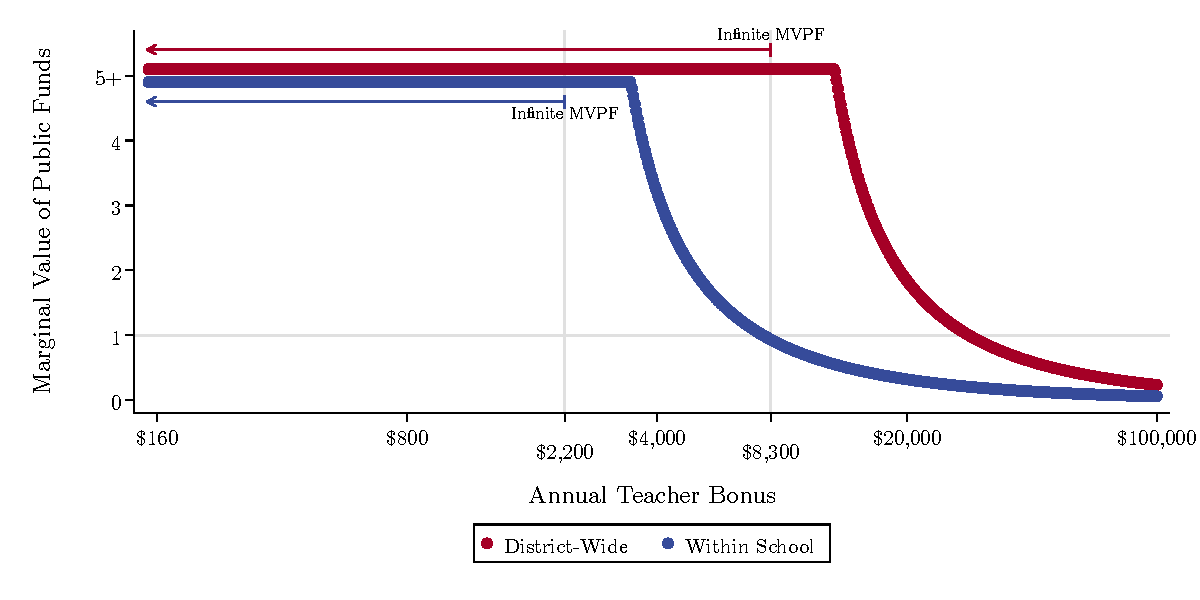
\includegraphics[width=.9\textwidth]{Working_Paper/test_figures/05_MVPF.pdf}
    \caption{Compensating Teachers for Reallocations Could Have Enormous Welfare Impacts}
    \label{fig:mvpf}
    \floatfoot{Note: This figure shows the marginal value of public funds for teacher bonus programs of different sizes (for either the within-school or district-wide reallocation). Values are capped at 5 on the figure, the range for which the MVPF is infinite is indicated with arrows, and the x-axis shown on a log scale. }
\end{figure}



The main takeaway from Figure \ref{fig:mvpf} is that for a broad range of bonus sizes the policy of reallocations and bonuses has an infinite MVPF. An infinite MVPF occurs when the net cost of the program is negative and the benefits are positive. In other words the district would be \textit{making} money by paying to reassign teachers---and would be increasing student earnings in the process. For the district-wide reallocation, the MVPF is infinite for a bonus of up to \$8,300, and it is infinite for bonuses up to \$2,200 for the within-school reallocation. This second number is particularly striking because despite being noninvasive the within-school reallocation is still generating substantial gains. 

A second important insight from Figure \ref{fig:mvpf} is that even when the MVPF is not infinite it is still large even for very costly bonus programs. For example, for the district-wide reallocation, a bonus program of paying \textit{every teacher} in the district \$20,000 to participate in the reallocation would still have an MVPF of roughly 2. In other words, it would generate \$2 of present valued earnings gains for every dollar spent on bonuses. This is a marked pay increase -- equivalent to a one-third salary increase for a teacher in the 2010-11 school year with 10 years of teaching experience and the middle tier of education in the district's collective bargaining agreement. 

Note that some of these bonus policies may not be incentive compatible, but other research suggests that reallocations with large and even infinite gains could be attainable. For example, while \$20,000 may sounds enormous, it amount was shown to be more than enough inducing teachers to move to very low performing schools in a large randomized controlled trial \citep{glazerman2013transfer}.
On the other hand, it's likely that almost all of the within-school reallocation are incentive compatible for most bonuses. First this is because teachers seem to care much more about which school they teach at than which class they teach---in large part because of commuting \citep{bates2022teacher}---and this is not affected in the within-school reallocation. Furthermore, in the within-school reallocation most teachers do not even switch classes, suggesting that the utility impact of the reallocation would be particularly small.


Taken together the teacher bonus thought experiment suggests that the large gains from reallocations are more than an impossibility. Although some teachers would be worse off because of certain reallocations, generating structures that appropriately compensate them for teaching to their comparative advantage could generate tremendous gains. In fact, many of the policies we explore generate large enough earnings gains to students to justify lavish teacher bonuses on the grounds of added tax revenue alone.


\section{Conclusion and Implications for Policy}
This paper set out to answer two questions: When does heterogeneity matter for maximizing a social objective in general? And how large are the welfare gains from using heterogeneous estimates for refining education policy in particular? We employed and extended tools from public finance to think about aggregating teacher effects on multidimensional outcomes and heterogeneous student types into welfare relevant statistics and implemented them in the context of a large urban school district. In reallocation exercises, using information about both multidimensionality and heterogeneity produce up to double the gains for test scores or for later-life outcomes relative to using standard measures that assume teachers have homogeneous impacts on students, and which focuses on one student outcome rather than two. This highlights the importance of incorporating such information into welfare considerations and policy.

We conclude by exploring three policy trade-offs that our results highlight and discussing possible directions for continued inquiry.


In the specific education value added context, our results highlight the power of comparative advantage relative to other policy proposals. Historically researchers have benchmarked the importance of teacher value added with the a policy ``deselecting'' (i.e., firing) low-performing teachers \citep[see][]{hanushek2009teacher,hanushek2011economic,chetty2014measuring2,Delgado2020}. Although deselecting 5\% of teachers with the lowest value added could produce large gains, there are concerns about the ethics of mistakes \citep{staiger2010searching} and the implications for teacher labor markets \citep{rothstein2015teacher}, in the sense that it is not obvious who the replacement teachers will be, and their own teaching effectiveness. An interesting implication of our results, however is that by relaxing the traditional assumptions of constant effects and equal class sizes we can reallocate rather than release teachers. In our setting a district-wide reallocation would produce gains more than three times larger than the gains from deselecting 5\% of teachers. Furthermore, because deselection using standard value added penalizes teachers who happen to be allocated to worse-matched classes, reallocations prevent incorrect dismissals---16-19\% of those targeted. A reallocation-based policy would be less costly to teachers and more beneficial. A within-school reallocation would be even less costly, and would still generate 50\% of the gains from deselection. In other words, our results suggest that in some, and perhaps many, cases, teachers in the bottom 5-10\% need not be deselected, but rather provided an assignment that better matches their comparative advantage. In other cases, where absolute advantage is extremely low, deselection could still be an option


A second,  more general, policy-insight is that our theory can show policymakers how mean evaluations of existing policies may (or may not) apply to new policy considerations. For example, we show that mean-based welfare estimates can be biased when based on estimates that are not externally valid, or when there is a covariance between welfare weights and treatment effects. While our results clearly indicate the value of considering heterogeneity, even without information beyond the means, policymakers can use these conditions to assess the severity of the bias. For example, using estimates from an expansion of Medicaid to beneficiaries similar to those who are eligible in another state may be very reasonable, whereas assuming that both welfare weights and the elasticity of taxable income are homogeneous along the income distribution may not be. Furthermore, policy can be further improved by conditioning on the relevant dimensions of heterogeneity. Admittedly, using characteristics to condition the estimates often reduces precision---although this type of tradeoff between bias and variability is hardly unique to our setting.


A final policy consideration to be taken from our results at large. Since value added and other mean evaluations are useful in so many contexts, we hope many practitioners will extend the use of heterogeneous estimates. As they do our research can provide a framework for the gains from adding heterogeneity and which dimensions of heterogeneity and multidimensionality to add and which to ignore. While our results highlight striking patterns in how value added heterogeneity specifically may affect the long-term outcomes of students, we note that assessing the optimality of reallocation policies in the long run will depend on heterogeneity in the long-term effects. We think an important next step in this literature is directly assessing the effect of multi-dimensional measures of teacher quality on various life-long outcomes and particular the heterogeneity in these relationships across groups. 

Taking a step back, our results also highlight the value of testing for and estimating heterogeneous estimates of teacher impacts, and of causal effects more broadly. Whether it is allocating teachers to classes, assessing racial health disparities in care, comparing possible social services, or measuring the effects of firms on earnings growth, the mean is rarely enough to characterize the full question of interest. Although estimating and implementing these evaluations can be costly, researchers have their own comparative advantage in such analyses, and our results suggest enormous gains from finding ways to leverage that knowledge to improve allocation in public programs of many types.



\bibliography{citations}

\renewcommand\thefigure{\thesection.\arabic{figure}}  
\renewcommand\thetable{\thesection.\arabic{table}}  
\setcounter{figure}{0}  
\setcounter{table}{0}  


\appendix



\section{Additional Tables and Figures}



\begin{figure}[hbtp]
\centering
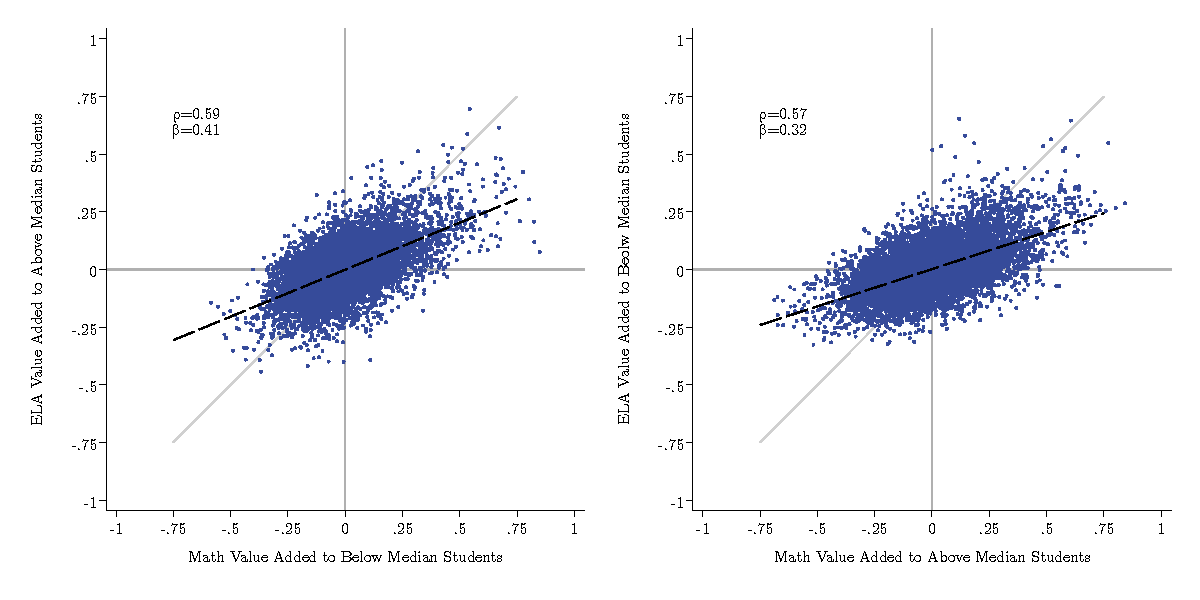
\includegraphics[width=.9\textwidth]{Working_Paper/test_figures/A2_crossVA.pdf}
    \caption{Cross-Subject and Cross-Type Value Added Is Much Less Correlated}
    \label{fig:A_va_est}
    \floatfoot{Note: This figure shows our heterogeneous estimates of teacher value added on both English Language Arts (ELA) and Math test scores. Note that in this Figure Math and ELA scores are plotted against each other. Each dot represents one teacher-year estimate of value added on high- and low-scoring students. The correlation coefficients is for the entire population stacked by year. The dotted line shows the line of best fit with the slope reported. For reference a line with slope one is plotted in the background. }
\end{figure}


\begin{figure}[htpb]
\centering
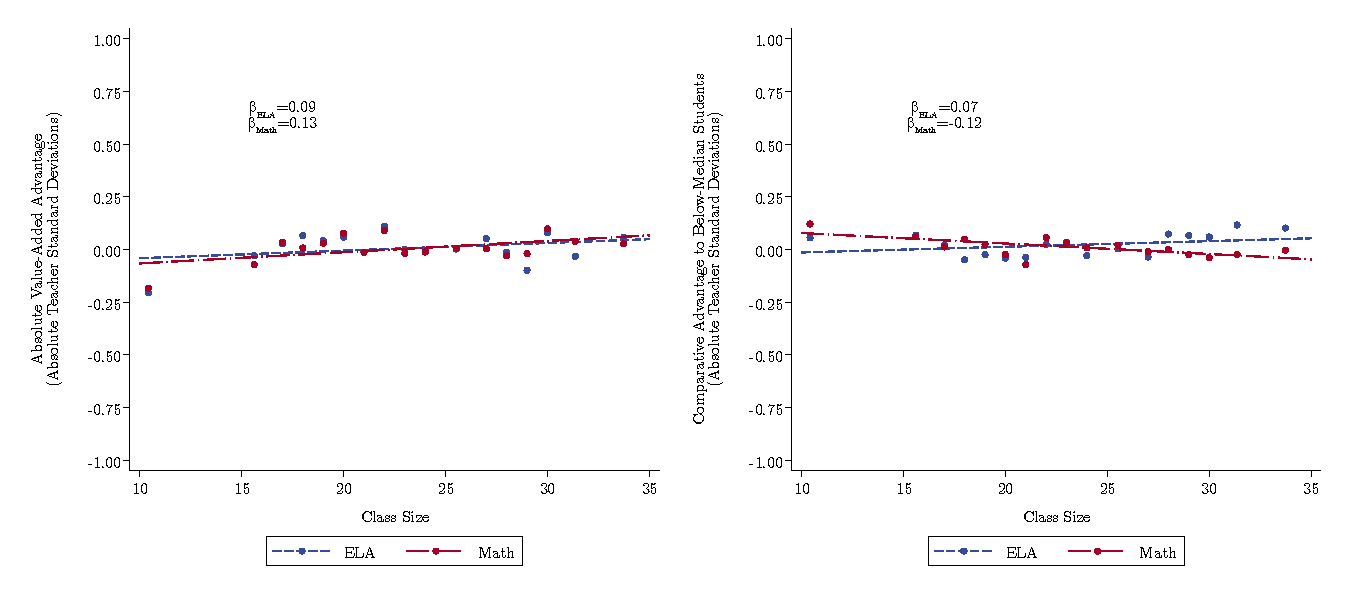
\includegraphics[width=.9\textwidth]{Working_Paper/test_figures/02_class_size.pdf}
    \caption{Value Added Only Varies Somewhat Across Class Sizes}
    \label{fig:squo2}
    \floatfoot{Note: This figure shows how our heterogeneous estimates of teacher value added on both English Language Arts (ELA) and Math test scores relate to class composition. The panel on the left shows teacher absolute advantage (average of value added on above- and below-median students) and the panel on the right shows the comparative advantage (difference of value added on below-median students minus value added on above-median students). Both panel plot the ventiles of value added (measured in teacher standard deviations in absolute advantage) over the share of number of students in each class. Both $\beta$ report the change from a 25-student change in class size. }
\end{figure}




\begin{figure}[hbtp]
\centering
    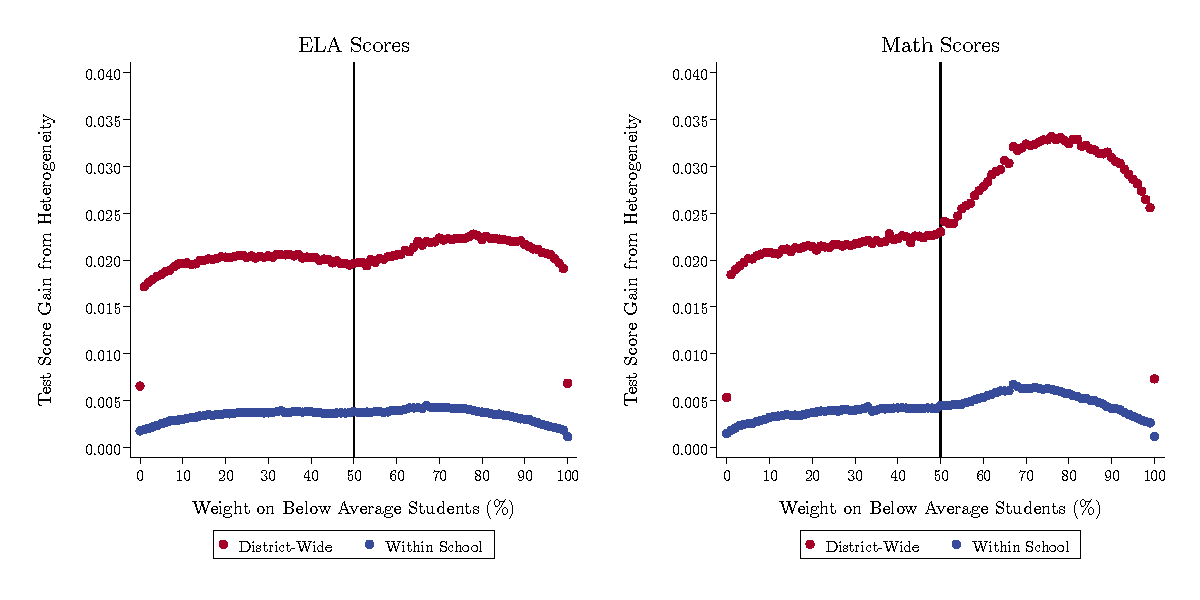
\includegraphics[width=.9\textwidth]{Working_Paper/test_figures/03g_reallocation.pdf}
    \caption{Test-Score Gains from Using Heterogeneity}
    \label{fig:equity3}
    \floatfoot{Note: This figure shows the test scores gains from using our measures of heterogeneous value added to make allocations relative to standard measures over various social preferences. }
\end{figure}


\begin{figure}[htpb]
\centering
\begin{subfigure}{\textwidth}
\centering
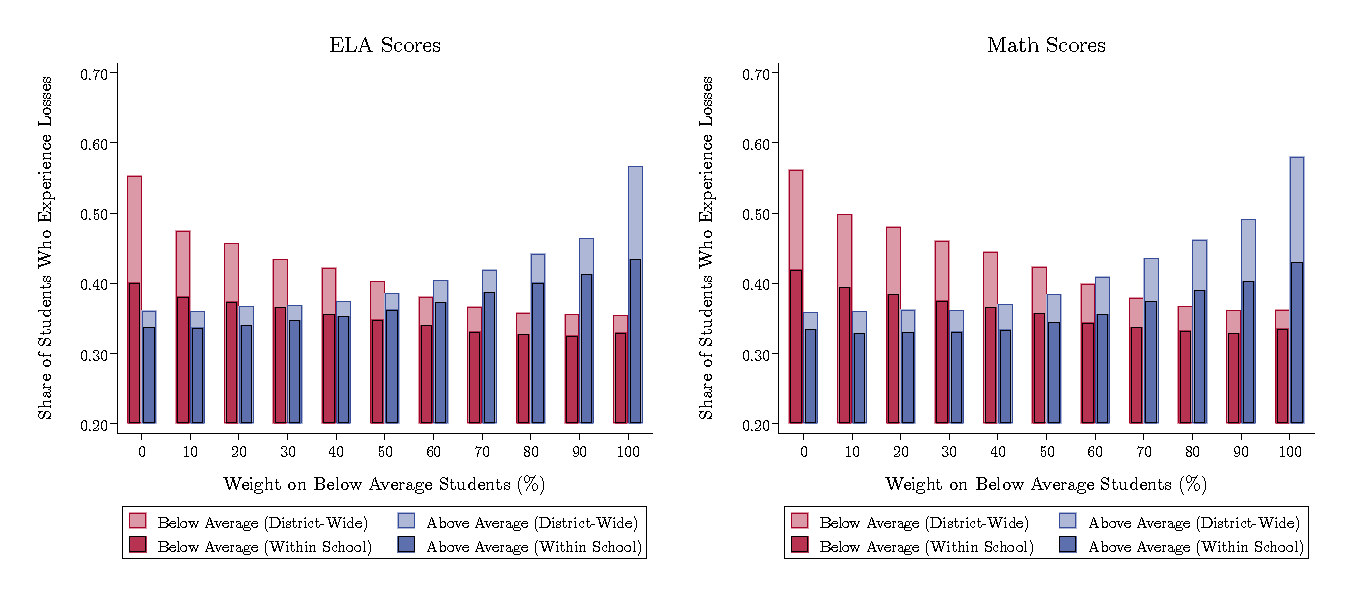
\includegraphics[width=.9\textwidth]{Working_Paper/test_figures/A4a_winlose.pdf}
    \caption{Share of Students Harmed}
 
\end{subfigure}

\begin{subfigure}{\textwidth}
\centering
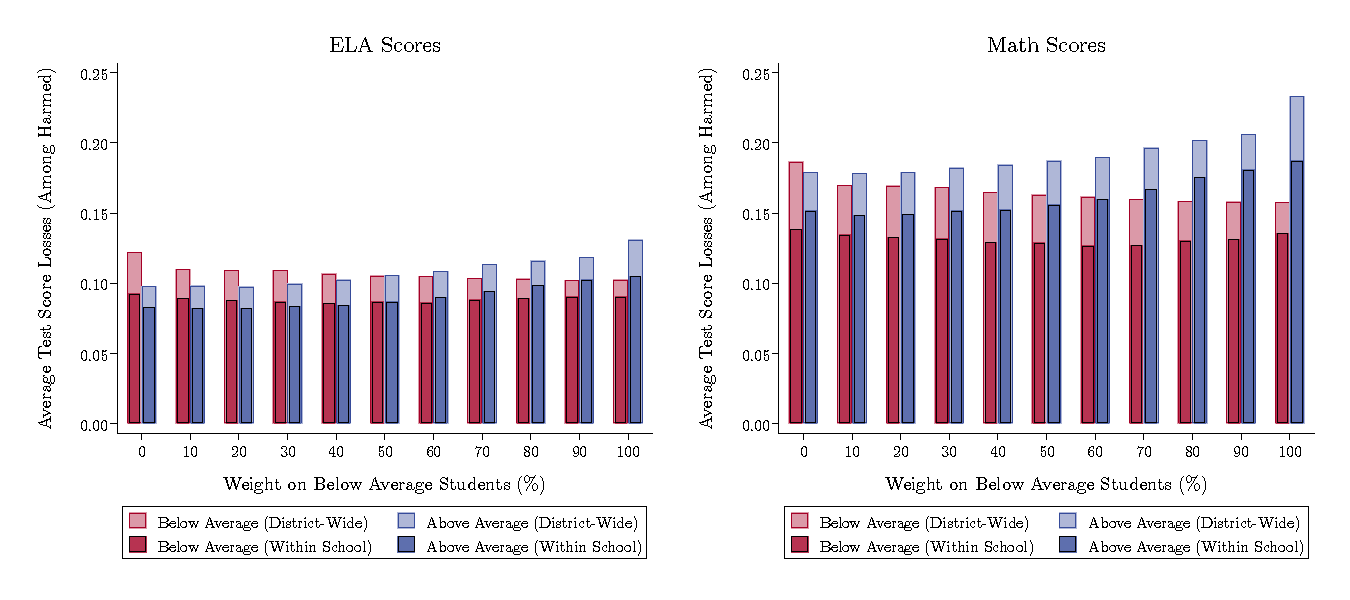
\includegraphics[width=.9\textwidth]{Working_Paper/test_figures/A4b_losssize.pdf}
    \caption{Mean Score Change among Harmed Students}
 
\end{subfigure}

    \caption{While Reallocations Help Many Students, They Will Harm Others}
    \label{fig:harms}
    \floatfoot{Note: This figure shows information about which students are made worse off by the reallocations. Panel (a) reports the share of students whose scores would be lowered by each reallocation and Panel (b) reports the average change in scores among those harmed.}
\end{figure}



\begin{figure}[hbtp]
\centering
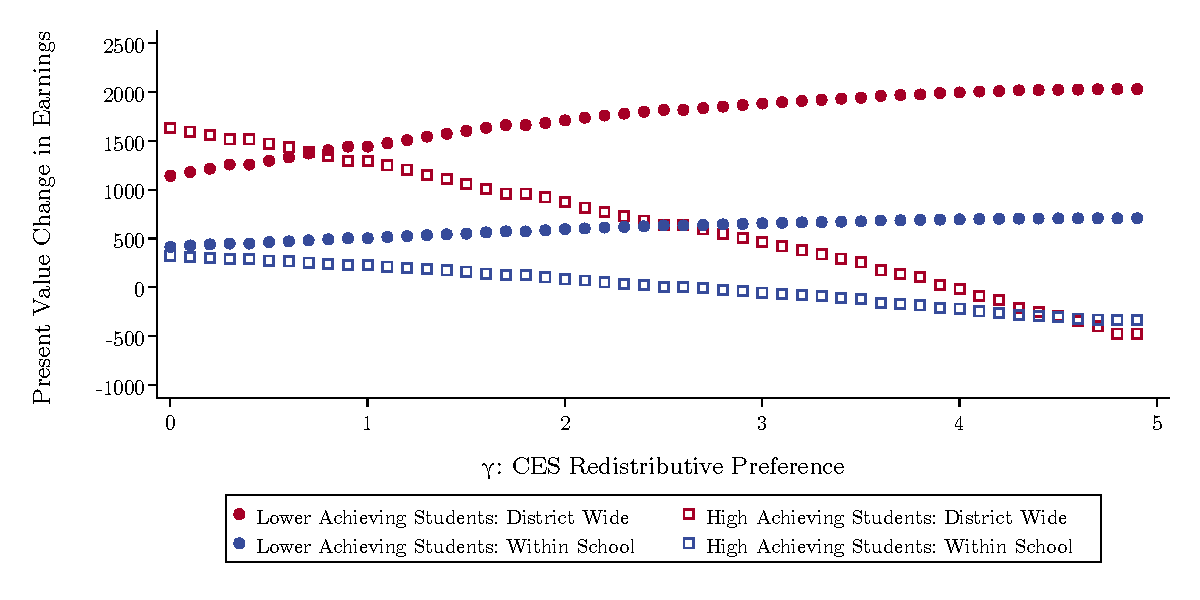
\includegraphics[width=.9\textwidth]{Working_Paper/test_figures/A5_CES.pdf}
    \caption{Comparing to a CES Benchmark}
    \label{fig:ces}
    \floatfoot{Note: This figure shows the present-value earnings gains from optimal reallocations based off of continuous CES preferences over student types rather than discrete preferences between high and low achievers.}
\end{figure}


\section{Theory Appendix}
\label{theory_appendix}

\subsection{From Test Scores to Welfare Details}
\label{definition_details}
Below is a more detailed version of definition \ref{def_welfare_change}
   \begin{proof}
    \label{def_welfare_change_detailed}
    If a change in an individual's outcomes $\bm{Y}_i$ only impacts the utility and welfare weights of that individual $i$, then for a given score function $S$, the expected change in welfare $  \Delta \accentset{\sim}{\mathcal{W}}^j$ from the status quo policy ($j=0$) to policy $j$ is 
    \begin{align*}
           \Delta \accentset{\sim}{\mathcal{W}}^j&\equiv   \E[\mathcal{W}^j|\bm{S}^j] - \E[\mathcal{W}^0|\bm{S}^0]  \\
             &  = \sum_{i=1}^n \E[\psi^j_i U^j_i |S_i^j] - \E[\psi^0_i U^0_i |S_i^0] \\ 
           &  = \sum_{i=1}^n \frac{\E[\psi^j_i U^j_i |S_i^j] - \E[\psi^0_i U^0_i |S_i^0]}{\Delta S^p_i} \Delta S^p_i \\ 
          &   \equiv \sum_{i=1}^n \gamma_i(S_i^j, S_i^0) \Delta S^p_i 
    \end{align*}


\end{proof}

    The last line is simply redefining the first term as a test score welfare weight $\gamma_i(S_i^j, S_i^0)$. $\bm{S}^j$ is the vector of test scores for every student under policy $j$. This means the expectations on the first line are conditional on the entire vector of test scores. This means the relationship between test scores and utility is fully flexible, and each student's utility can be uniquely impacted by a given test score change. Note that $\gamma_i$ is an average over test score points for a given student, not an average across students. To understand this term, it is helpful to think through a simple example. Suppose  $ \E[\psi^j_i U^j_i |S_i^j] = S_{it}$ for all students. That is, expected welfare is linear in test scores. In this case,  $\gamma_i(S_i^j, S_i^0) = 1$ because all students gain 1 util per score over the entire range of scores, and test scores are equivalent to welfare. Although welfare weights are often based off of earnings or earnings ability, the implication of definition \ref{def_welfare_change} is that we can theoretically apply weights to a short term outcomes like test scores, rather than utility, and still have an unbiased estimate of welfare. Of course, in practice, getting individual weights is likely impossible. The later theory sections address the best way to overcome this problem with conditional aggregation, but definition \ref{def_welfare_change} provides a ground truth reference that incorporates a large amount of of potential heterogeneity, individual differences. 
 
\subsection{Welfare Weighting the ATE}
\label{appendix_ww_ate}
    Using a similar approach to  \cite{Keyser_2020}, the following equation shows how it is possible to estimate welfare from an average treatment effect if the proper weight is applied


    \begin{align}
           & \Delta \mathcal{W}^j \\
           &  = \int_0^1 \gamma_i(S_i^j, S_i^0) \Delta S^p_i \text{d}i\\
           & = \frac{\int_0^1 \gamma_i(S_i^j, S_i^0) \Delta S^p_i \text{d}i}{\int_0^1 \Delta S^p_i \text{d}i} \int_0^1 \Delta S^p_i \text{d}i \\
           & =  \Tilde{\gamma}^j ATE^j 
    \end{align}

    The trouble is that the first term, $\Tilde{\gamma}^j$ depends, not just on the test score welfare weights $\gamma_i$, but also on the joint distribution of those weights with the changes in test scores for policy j. It is a complex object that involves a deep understanding of the distribution of heterogeneous impacts resulting from policy $j$. If a policymaker already has this deep knowledge, it is not clear how much giving them the average treatment effect will help.



    \subsection{Theorem \ref{thm_bias_nc} proof}
    \label{th_bias_nc_proof}
    \begin{proof}
    \begin{align*}
        \textbf{Average Bias}_{ATE} &= \frac{\Delta \accentset{\sim}{\mathcal{W}}^j}{n} - \E[\gamma^p] \widehat{ATE} \\
       & =   \frac{1}{n}\sum_{i=1}^n \gamma_i(S_i^j, S_i^0) \Delta S^p_i - \E[\gamma^p] \widehat{ATE}  \\
        & =  \E[\gamma^p \Delta S^p] - E[\gamma^p] \widehat{ATE}  \\
       & =  \E[\gamma^p] \E[\Delta S^p] + \Cov(\gamma^p, \Delta S^p) - E[\gamma^p] \widehat{ATE}  \\
       & = \Cov(\gamma^p, \Delta S^p) +\E[\gamma^p] \left (\E[\Delta S^p]-\widehat{ATE} \right )
    \end{align*} 
    The first line is how we are defining bias. It is the benchmark with individual heterogeneity minus our common estimator of the mean welfare weight and the average treatment effect. The second line comes from definition \ref{def_welfare_change}. The third line comes from recognizing that the first term in line two is the population average, or expectation, of $\gamma^p \Delta S^p$. The fourth line uses the general definition of covariance, that is $\Cov(X,Y) = \E[XY] - \E[X]\E[y]$. The last line just rearanges the terms. 
    \end{proof}

\subsection{Averate Treatment Effect Bias Explained}
\label{ATE_bias_appendix}

    The specific source of average treatment effect bias we are consider can be a concern for any  policy $j$ that involves assigning specific sub-treatments $d$ (teachers) to subsets of the population of size $K^j_d$ (classes). First note that the average treatment effect is the following weighted average of sub-treatment effects $ATE^j_d$
    
    \begin{equation*}
       ATE^j = \frac{1}{n}\sum_d K^j_d ATE^j_d
    \end{equation*}  

    The bias comes in from incorrect estimates of the average sub-treatment effect (teacher impact) $ATE^j_d$ characterized by the following 

    \begin{align*}
        ATE^j_d - \widehat{ATE}^j_d & = \frac{1}{K^j_d} \sum_{i = 1}^{K^j_d} \Delta S_i^d - \frac{1}{K^0_d} \sum_{l = 1}^{K^0_d} \Delta S_l^d
    \end{align*}
    
    % when is the second thing not a problem 
    Here we can see the bias comes from different individual impacts between the existing class and the class in the policy counterfactual. It is helpful to think through the two cases where this difference goes to zero. First, if there is no treatment effect heterogeneity. For example, a teacher impacts all students equally on average and so $\Delta S_i^d = \Delta S_l^d \quad \forall \quad i,l$. Second, even if there is treatment effect heterogeneity, if the classes have similar characteristics the means may still be the same. For example, a teacher may be very bad at teaching English language learners (ELA). However, if both classes have the same fraction of ELA students, the teacher's mean impact will be the same. 

    \subsection{Conditional Average Treatment Effect Bias Explained}
    \label{CATE_bias_appendix}

     The bias in the second term will be lower after conditioning when 
    
    \begin{align}
        & \E[\Delta S^p]-\widehat{ATE} > \sum_{x} P_x \left( \E[\Delta S^p|x]-\widehat{CATE(X)} \right) 
    \end{align}

    As in the previous section, we can zero in on a specific teacher or sub-treatment and see that, for a given teacher, conditioning reduces bias when 
    
    \begin{align}
     & ATE^j_d - \widehat{ATE}^j_d \\
        &  = \frac{1}{K^j_d} \sum_{i = 1}^{K^j_d} \Delta S_i^d - \frac{1}{K^0_d} \sum_{l = 1}^{K^0_d} \Delta S_l^d \\
        & > \sum_X P^j_{dx} \left( \frac{1}{K^j_{dx}} \sum_{i = 1}^{K^j_{dx}} \Delta S_i^d - \frac{1}{K^0_{dx}} \sum_{l = 1}^{K^0_{dx}} \Delta S_l^d \right) \\
        &  \sum_X P^j_{dx} \left( \widehat{ATE}^j_{dx} - \widehat{ATE}^0_{dx}  \right) 
    \end{align}

    The left side is the difference in mean treatment effects between the baseline class and the counterfactual class, as described above. The right hand side is the difference in the mean treatment effects for a given x, weighted by the portion of students in the counterfactual class in group x. Bias in this case comes from differences within a group x between the baseline and counterfactual treatment effects. There is no longer any bias from differences in the fraction of students with characteristics x. If a teacher is worse at teaching struggling students, for example, and their new class has many more struggling students, the left hand side will overestimate their impact on the new class. The right hand side will only be biased if there is variation within performance groups in both the teachers impact and the student compositions. For example, teachers may have different impacts on students based on race, even within a pretest group, and racial composition could differ across class \citep{Delgado2020}.


\section{Data Appendix} \label{data}


\section{Value Added Estimation Details} \label{estimation}


    The above discussion shows the theoretical importance of measuring test score heterogeneity, but of course, measuring heterogeneity increases the variance of estimates. Weather or not it can be effectively measured to improve policy analysis is a practical empirical question. Below we cover two different methods for measuring test score heterogeneity, but first, a quick review of our benchmark traditional value added estimation. 


    %%%%%%%%%%%%%
    % Estimators
    \subsection{Estimators}
    \subsubsection{Standard Value Added}

    In order to reference our estimates against an up to date and rigorously tested value added approach, we follow the baseline practices used in \citet{chetty2014measuring1} and implement it using the associated Stata package \citep{vam_stata_ado}. The general approach of these authors is as follows. First regress test scores $S_{i,t}$ on controls $X_{i, t}$ which gives test score residuals $A_{it}$. This is obtained from a regression on test scores of the form 
    
    \begin{equation}
        S_{i,s,t} = \alpha_{j(i,s,t)} + \beta_s X_{i, t} + \epsilon_{i,s,t}
    \end{equation}

    Where $X_{i, t}$ includes cubic polynomials in prior year test scores in math and ELA, those polynomials interacted with student grade level, ethnicity, gender, age, lagged suspensions and absences, indicators for special education and English language learner status, cubic polynomials in class and school-grade means of prior test scores in both subjects each interacted with grade, class and school means of all the other covariates, class size and type indicators, and grade and year dummies\footnote{The covariates match those used in \citep{chetty2014measuring1} closely. Means and standard deviations of the underlying variables appear in Appendix Table \ref{}.}.  $j(i, t)$ is the index for the teacher who has student $i$ in her class at time $t$, so $\alpha_{j(i, t)}$ are year-specific teacher fixed effects.

    Next, we average the residuals within each class year to get 
    \begin{equation}
        \bar{A}_{jt} = \frac{1}{n} \sum_{i \in {i: j(i, t) = j}} A_{it}
    \end{equation}

    The last step is to use the average residuals in every year but year t, denoted $\mathbf{A}_j^{-t}$, to predict $\bar{A}_{jt} $. Specifically, we choose coefficients $\psi = (\psi_i, ..., \psi_{t-1})$ to ``minimize the mean squared error of the forecast test scores \citep{chetty2014measuring1}"

    \begin{equation}
        \psi = \argmin_{\psi} \sum_j \big(  \bar{A}_{jt} - \sum_{s = 1}^{t-1} \psi_s \bar{A}_{js} \big)^2
    \end{equation}

    This then gives the estimate for teacher j's value added in year t of 
    \begin{equation}
        \hat{\mu}_{jt} = \psi'\mathbf{A}_j^{-t}
    \end{equation}

    \subsubsection{Binned Estimator}
    A simple way to add heterogeneity into this model is to include an indicator for each student's type and estimate teacher affects separately for each type. This gives each teacher an estimate for each student type. We separate students into above and below median prior year test score bins. All of the above math works out essentially the same except we now have twice as many parameters to estimate. We now estimate residuals from the equation

     \begin{equation}
        S_{i,t} = \alpha_{j(i,b, t)} + \beta X_{i, t}
    \end{equation}

    where $j(i,b, t)$ indicates if student i is assigned to teacher j in bin b at time t. Next we group residuals for teacher, year, bin, 

    \begin{equation}
        \bar{A}_{jBt} = \frac{1}{n} \sum_{i \in {i: j(i, B, t) = j}} A_{it}
    \end{equation}

    and we do the leave-one-out estimator with teacher bin estimates across years 

    \begin{equation}
        \psi = \argmin_{\psi} \sum_j \big(  \bar{A}_{jBt} - \sum_{s = 1}^{t-1} \psi_s \bar{A}_{jBs} \big)^2
    \end{equation}

    This then gives the estimate for teacher j's  bin B Value added in year t of 
    \begin{equation}
        \hat{\mu}_{jBt} = \psi'\mathbf{A}_{jB}^{-t}
    \end{equation}

    We also apply statistical shrinkage, using the variance within each bin so that if the variance of one bin is higher it does not get shrunk more relative to the other bins. 


    % cut this. Leaving this comment as a placeholder for reference
    % \subsubsection{Non-Parametric Estimator}

         %%%%%%%%%%%%%%%%%%%%%%%%%%%%%%
        % Aggregating estimates 
        \subsection{Aggregating Estimates}
        The above method gives multiple estimates for each teacher's impact on the different types of students. For specific policy interventions, like teacher reassignment, these can be combined by summing up the conditional expected treatment with the conditional average welfare weight such as the weights described in theorem \ref{thm_cond_bias}. 

        However, in some cases,  value added is also used for general teacher ranking and assessment. If teacher heterogeneity is significant, is there still a way to objectively rank teachers according to a particular set of heterogeneous welfare weights? There is not a perfect single solution since their impact depends on the class or policy environment. However, one solution that puts teachers on an even playing field is to rank teachers on the expected welfare impact they would have on an average representative class, rather than on the average impact on test scores for the class they have, which may depend on class composition, which is outside of the teacher's control and does not reflect their welfare impact.
        
        
        In the discrete setting, let $\bar{\omega_k}$ and $\gamma_k$ be the average proportion of students in group k and the welfare weight for group k respectively. Let $\alpha_{j,k}$ be teacher j's group specific value added for group k. Than we can aggregate their group specific test scores as 
        \begin{equation}
        \label{agg_equation}
            VA_j = \sum_k \gamma_k \bar{\omega_k} \alpha_{j,k}
        \end{equation}
        
        This gives the welfare benefit a teacher would have on an average class. This is the same as $A_j$ from definition \ref{hetero_decomp}. Now, choosing the average class composition for every teacher may or may not be the right normative choice. Suppose that a teacher has a big comparative advantage with high scoring students in a district with, on average, very high scoring students, but their class is primarily low scoring. What is the right way to assess their performance? They may not be bad relative to their well matched peers, which the above metric could tease out, but they may still in fact be doing a poor job helping the students they have, which the above metric ignores. This emphasizes that in a world of heterogeneity, no metric will be perfect. However, equation \ref{agg_equation} does help to rank teachers based on what is under their control. 
        


\section{Validation and Robustness of Heterogeneous Estimates} \label{robustness}


\begin{itemize}
    \item Text about forecast unbiasedness
\end{itemize}


\begin{figure}
    \centering
    \includegraphics[width=.35\textwidth]{example-image-b} \hspace{2em}
    \includegraphics[width=.35\textwidth]{example-image-b}
    \caption{Measures of Comparative Advantage are Forecast Unbiased}


    \label{fig:robust1}
\end{figure}


\begin{itemize}
    \item Text about persist/stability
    \item $\hat{\gamma}^g_{j,t} = \rho^g \hat{\gamma}^g_{j,t-1} + u_{j,t}$
\end{itemize}


\begin{figure}
    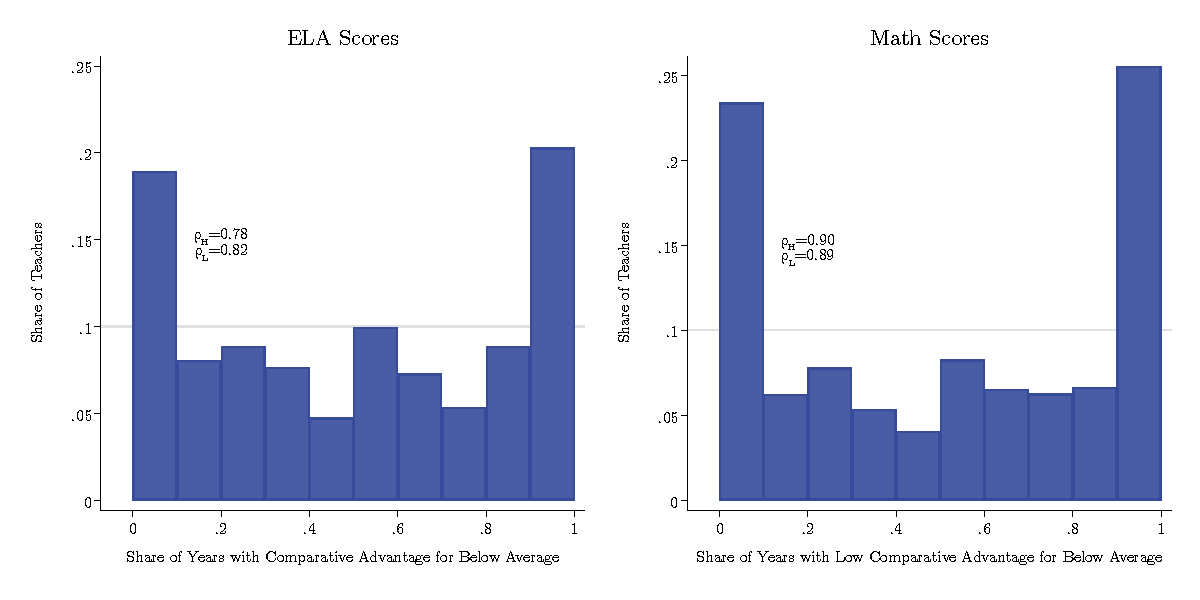
\includegraphics[width=\textwidth]{Working_Paper/test_figures/02b_hist.pdf}
    \caption{Measures of Comparative Advantage Persistent}
    \label{fig:robust2}
\end{figure}


In addition to these standard exercises we leverage the longitudinal nature of our data to show that our heterogeneous estimates capture the same correlations with long term outcomes as do standard value added does---despite being identified off of only half of the students.  In the spirit of \citet{chetty2014measuring2}, we focus on five main outcomes: high school graduation, college enrollment in the year after twelfth grade (two-year, four-year, and any), and completion of a bachelors degree within six years of (anticipated) high school graduation. If our heterogeneous estimates corresponds to future outcomes in a similar way to standard value added, then the predictive power has not been diminished and the estimated effects are fitting on true value added rather than idiosyncratic noise. 

To test the predictive power of value added, we regress each outcomes teacher value added and the controls from equation \ref{} in a student-subject-grade level regression. For the binned estimates, we include terms for the high- and low-bin value added interacted with an indicator for whether the student is a high scoring: 
    \begin{align}\label{long}
        y_{i,j,s,t} &= \tau_{VA} \hat{\gamma}^{VA}_{j,s,t}\mathds{1}(k_i = g) + \beta_2 X_i + \nu_{i,j,s,t} \\ \nonumber
        y_{i,j,s,t} &= \sum_{g=H,L} \tau_{g} \hat{\gamma}^g_{j,s,t}\mathds{1}(k_i = g) + \beta_3 X_i + \nu_{i,j,st}
    \end{align}
\noindent   This is analogous to treating the each teacher-subject-bins as a separate class where the coefficients on value added indicate the predictive power of high-bin value added in each subject on high-scoring students' outcomes  and low-bin value added on low-scoring students' outcomes. 

Figure \ref{fig:robust3} reports the results from the regression in equation \ref{long} on each outcome variable. Our results show striking similarities between traditional value added and our estimates, despite the fact that we split our sample to estimate above- and below median effects. Surprisingly, none of the measures are predictive of high school graduation. One explanation for this might be that SDUSD has an unusually high graduation rate, averaging 90 percent for our sample, creating ceiling effects. While not statically significant, standard value added and both of our binned estimates track closely with an increase in any college, primarily from four year college with potentially a drop in two year college, and an increase in a bachelor's degree within 6 years. We can also see that the standard errors for each student group are not actually much bigger than for the mean as a whole suggesting that the variance is loading on this achievement dimension. On a whole these effects are similar with those in \citet{chetty2014measuring2} and \citet{pope} for traditional value added. 


\begin{figure}[hbtp]
\centering
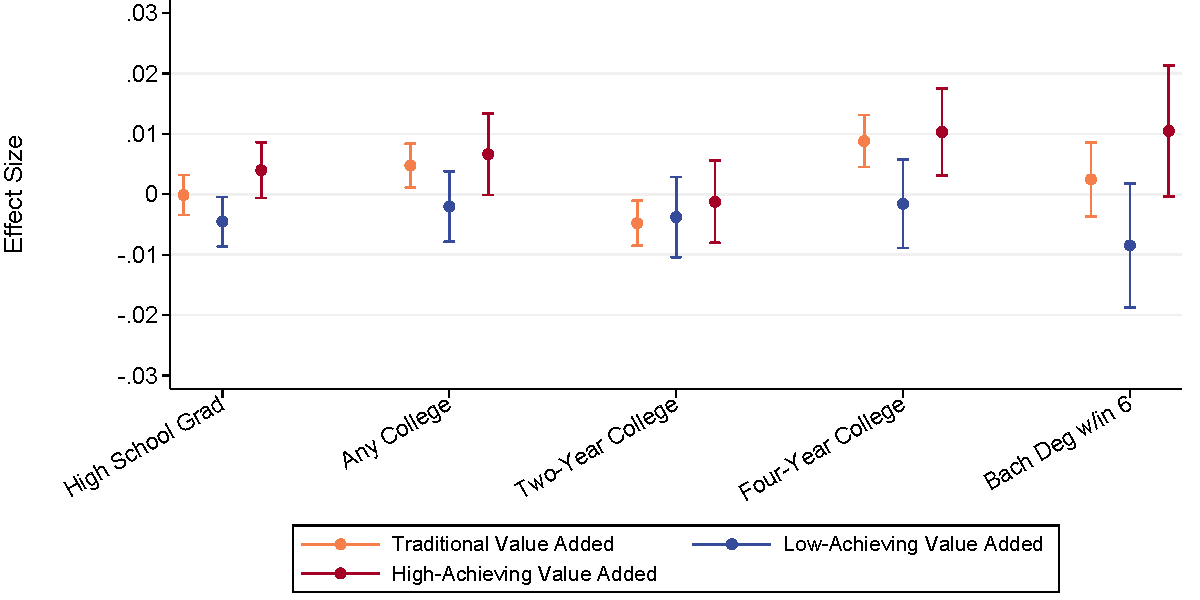
\includegraphics[width=.9\textwidth]{Working_Paper/WP_Figures/fig2b_longterm.pdf}
    \caption{Our Estimates Predict Long Term Effects as Well as Standard VA}
    \label{fig:robust3}
    \floatfoot{Note: This figure compares the effect of different measures of teacher value added on long-term outcomes. All regressions follow equation \ref{long} and include all controls from the value added estimation. For the outcomes, High School Grad is an indicator for whether the student graduated from high school, Two Year College is an indicator for whether the student enrolled in a two-year college within a year following high school graduation, Four-Year College is an indicator for whether the student enrolled in a four-year college within a year following high school graduation, and Any College is an indicator for either Two Year College or Four-Year College. Finally, we model an indicator for whether the student obtained a Bachelor's degree within six years of high school graduation.}
\end{figure}

Although imprecise, these effects point to patterns in college enrollment that are independently interesting beyond this validation exercise. For example, the effect on two-year college enrollment is higher for below-median students, which makes sense if they are more likely to be on the margin of not going to any college. On the other hand, for high-scoring students, well matched value-added may decrease the probability of two-year college enrollment and increase in the probability of four-year college enrollment. These patterns are consistent with well-matched teachers increasing the quality of post-secondary education, moving students on one margin from no college to two-year colleges and on another margin from two-year colleges to four-year colleges.
    


\section{Reallocation Problem and Solution Concept} \label{optimization}


%%%%%%%%%%%%%%%%%%%%%%%%%%%%
% citation and appendix %%%%%%


\end{document}